% Prefer the fallback `article` class unless an explicit marker enables the
% vendor class. To force the vendor class create an empty file named
% `USE_VENDOR_CLASS` in the project root. This prevents class-provided package
% load-order issues (e.g., cleveref vs hyperref) during automatic builds.
\IfFileExists{zHenriquesLab-StyleBioRxiv.cls}{%
  \IfFileExists{USE_VENDOR_CLASS}{%
    \documentclass[times, twoside, watermark]{zHenriquesLab-StyleBioRxiv}
  }{%
    \documentclass[11pt]{article}
    \usepackage[margin=1in]{geometry}
    % Provide compatibility shims when the vendor class is absent (Overleaf/fallback)
    \usepackage{authblk}
    \providecommand{\leadauthor}[1]{}
    \providecommand{\shorttitle}[1]{}
    \providecommand{\corrauthor}[1]{}
    \providecommand{\Letter}{}
    \renewcommand\Affilfont{\small}
  }
}{%
  \documentclass[11pt]{article}
  \usepackage[margin=1in]{geometry}
  % Provide compatibility shims when the vendor class is absent (Overleaf/fallback)
  \usepackage{authblk}
  \providecommand{\leadauthor}[1]{}
  \providecommand{\shorttitle}[1]{}
  \providecommand{\corrauthor}[1]{}
  \providecommand{\Letter}{}
  \renewcommand\Affilfont{\small}
}

% Core packages
\usepackage{graphicx}
\usepackage{booktabs}
\usepackage{multirow}
\usepackage{amsmath}
\usepackage{amssymb}
\usepackage{microtype}
\usepackage{needspace}
\usepackage[section]{placeins}
\usepackage{caption}
\usepackage{multicol}
\usepackage{tikz}
\usepackage{tcolorbox}
\usetikzlibrary{arrows.meta,positioning,fit,calc}
\usepackage[colorlinks=false,pdfborder={0 0 0},breaklinks=true]{hyperref}
\usepackage{cleveref}
\usepackage{longtable}
\usepackage{array}

% Compatibility shims for environments defined only by the vendor class
\makeatletter
\@ifundefined{keywords}{%
  \newenvironment{keywords}{\noindent\textbf{Keywords:} }{\par}%
}{}
\@ifundefined{endacknowledgements}{%
  \newenvironment{acknowledgements}{\section*{Acknowledgements}}{}
}{}
\makeatother

% Note: if you need journal-specific styling, provide the class file locally
% (ignored by git) or switch to the journal template during submission.

\leadauthor{Erzurumluoğlu}

\begin{document}

\title{Pan-Cancer Identification of Triple-Target Combinations Reveals a Recurrent STAT3-Centric Survival Architecture}
\shorttitle{Pan-Cancer Triple-Target Combinations}

% Use a single, robust author block compatible with both the vendor class
% and the fallback article+authblk combination. The corresponding author
% email is included via \thanks{} to avoid class-specific macros.
\author{Roy Erzurumluoğlu\thanks{Corresponding author: \href{mailto:roy.erzurumluoglu@gmail.com}{roy.erzurumluoglu@gmail.com}}$^{,}$\thanks{ORCID: \href{https://orcid.org/0009-0000-9523-881X}{0009-0000-9523-881X}}\\
  Independent Researcher, The Netherlands.\\
  {\small Previously: Maastricht University, Faculty of Science and Engineering, Maastricht, The Netherlands.}}

\maketitle

\begin{abstract}
Across 77 cancer types, analysis of DepMap CRISPR essentiality data and OmniPath signaling networks reveals a recurrent triple-target architecture: a convergent survival hub (predominantly STAT3, present in 78\% of cancer types), cell-cycle effectors (CCND1, CDK4/6), and cancer-specific oncogenic drivers. This three-component structure parallels the tri-axial inhibition principle demonstrated experimentally in pancreatic cancer, where simultaneous blockade of three independent signaling axes prevented resistance for $>$200 days~\cite{Liaki2025}. Using ALIN (Adaptive Lethal Intersection Network), a pipeline that infers cancer-specific survival mechanisms, identifies minimal hitting sets (MHS) covering all inferred mechanisms, and scores triple combinations for synergy, resistance risk, and toxicity, I evaluate predictions against 43 independently curated gold-standard clinical combinations: 44.2\% any-overlap, 30.2\% pair-overlap, and 7.0\% exact concordance ($p < 0.001$, permutation test). Third-target predictions for five FDA-approved doublets match clinical evidence in 5/9 cases (56\%; $p \leq 10^{-5}$). Independent pharmacological validation confirms that predicted target pairs exhibit significantly higher drug combination synergy in DrugComb v1.5 (ZIP: $\Delta = +2.59$, $p = 0.0001$; Bliss: $\Delta = +2.00$, $p = 0.011$). A dual-track analysis---comparing druggability-weighted (translational) and druggability-neutral (discovery) predictions across 76 cancers---reveals that conventional pharmacological weighting restricts the target landscape to 22 genes; removing all druggability priors expands this to 89 targets, a 4.0-fold increase. Eight cancers receive identical triples regardless of weighting, identifying the strongest convergence candidates; 73 discovery-only targets define a ranked drug-development agenda for emerging modalities (PROTACs, molecular glues, allosteric inhibitors). Degree-preserving network null tests confirm that STAT3's pan-cancer recurrence exceeds hub-degree expectation ($p < 0.05$), supporting biological rather than purely topological selection.
\end{abstract}

\begin{keywords}
cancer | drug resistance | triple-target combinations | combination therapy | DepMap | STAT3 | minimal hitting sets | precision oncology
\end{keywords}

\noindent\textbf{Corresponding author:} \href{mailto:roy.erzurumluoglu@gmail.com}{roy.erzurumluoglu@gmail.com}

\newpage
\twocolumn
\raggedbottom
\sloppy

% Aggressive float placement - reduce white gaps around figure*/table*
\renewcommand{\dbltopfraction}{0.9}      % up to 90% of page for top floats
\renewcommand{\textfraction}{0.07}       % min 7% text (default 20%)
\renewcommand{\dblfloatpagefraction}{0.7}% float-only pages need 70% fill
\setcounter{dbltopnumber}{2}             % allow 2 double floats per page top
\setcounter{topnumber}{3}
\setcounter{totalnumber}{5}

%TC:break main

\section*{Introduction}

Single-agent cancer therapies fail because tumors adapt: when one signaling pathway is inhibited, compensatory pathways sustain survival. This \emph{pathway shifting} is the fundamental mechanism of acquired drug resistance~\cite{Bergholz2021,Xin2024}. Combination therapy addresses this by simultaneously blocking multiple survival axes, but the vast combinatorial space makes rational design essential.

Liaki et al.~\cite{Liaki2025} demonstrated a solution in pancreatic ductal adenocarcinoma (PDAC): tumor cells maintain viability through three independent signaling nodes--\textbf{downstream} (RAF1), \textbf{upstream} (EGFR), and \textbf{orthogonal} (STAT3) to KRAS signaling. Ablating two nodes triggers compensatory activation of the third (e.g., RAF1+EGFR ablation activates STAT3 via FYN~\cite{Chougule2016,Zhang2020FYN}). Only simultaneous targeting of all three axes induced complete tumor regression with no resistance for $>$200 days; dual combinations failed~\cite{Liaki2025}.

This tri-axial inhibition principle provides a framework for combination therapy design, but generalizing it beyond PDAC requires answering a cancer-specific question: \emph{which genes, when targeted simultaneously, cover the inferred survival mechanisms for each cancer type?}

I present ALIN (Adaptive Lethal Intersection Network), a computational pipeline that addresses this question (\cref{fig:pipeline}). ALIN infers cancer-specific survival mechanisms from DepMap~\cite{Dempster2021} and OmniPath~\cite{Turei2026} data, identifies target combinations covering every inferred mechanism via \textbf{minimal hitting set (MHS)} optimization~\cite{VeraLicona2013,Murakami2017}, and scores triple combinations for estimated synergy, resistance risk, and toxicity. My contributions: (1)~discovery of a recurrent STAT3--cell cycle--oncogene target architecture across 77 cancer types that parallels the experimentally validated tri-axial principle; (2)~target-concordance evaluation against 43 independently curated gold-standard combinations ($p < 0.001$); (3)~independent pharmacological validation showing predicted target pairs exhibit significantly higher drug combination synergy in DrugComb v1.5; (4)~systematic hub-bias analysis and PageRank-normalized correction. The distinction between computationally derived triple-target combinations and experimentally demonstrated mechanistic tri-axiality~\cite{Liaki2025} is maintained throughout; disease-specific validation remains essential.

\section*{Methods}

\subsection*{Data sources}
I use DepMap~\cite{Dempster2021,Tsherniak2017} release 24Q4 (accessed January 2026) for gene dependency $D_{g,\ell}$ (Chronos score~\cite{Dempster2021} from CRISPRGeneEffect.csv), cell line metadata (Model.csv), and cancer type mapping via OncoTree (OncotreePrimaryDisease). OmniPath~\cite{Turei2026} provides the directed signaling network $G = (V, E)$ (accessed January 2026; cached for reproducibility). PRISM~\cite{Corsello2020} and GDSC~\cite{Yang2013,Iorio2016} supply drug sensitivity data for validation. All data versions and access dates are documented in VERSION\_INFO.md (Supplementary Methods, Section~S1).

\subsection*{Reproducibility}
Unless otherwise noted, results are reproducible given (i)~the fixed input dataset releases and access dates above, (ii)~the full parameter configuration listed in VERSION\_INFO.md, and (iii)~a fixed random seed for stochastic steps (random candidate baselines, permutation tests). All randomization-based $p$-values are estimated from the stated number of iterations and should be interpreted as Monte Carlo estimates.

\subsection*{Survival mechanism inference}
I infer cancer-specific survival mechanisms--heterogeneous objects representing independent routes by which tumor cells maintain viability--through four complementary approaches (mathematical definitions in Supplementary Methods~S2). I use ``survival mechanism'' rather than ``path'' as a collective term, since these objects have different semantics; the term ``path'' is reserved for directed OmniPath network paths below.

\textbf{1. Essentiality and selectivity.} A gene is essential if its Chronos score $< -0.5$ and selective if essential in $\geq$30\% of cell lines for that cancer type~\cite{Dempster2021,Behan2019}. Pan-essential genes ($>$90\% of all cell lines) are excluded. A threshold sensitivity sweep (500 configurations, 5 cancers) confirmed robustness (see Sensitivity).

\textbf{2. Co-essentiality modules.} I group genes into 3--15 co-essential survival modules by computing pairwise Jaccard similarity on binarized dependency profiles (essential/non-essential per cell line) and clustering the resulting distance matrix with Ward's hierarchical method~\cite{Pan2018}. I use Jaccard rather than Pearson correlation because the relevant structure is shared essentiality membership rather than continuous Chronos score magnitude; however, this binarization discards information about dependency strength. To quantify how much information is lost, I compared Jaccard-binarized vs.\ Pearson-correlation distance matrices across 10 cancer types ($\geq$74 cell lines each), clustering both with Ward's method for $k = 3$--$15$ and computing normalized mutual information (NMI) between the resulting partitions. Agreement was low (mean NMI = $0.20 \pm 0.07$; Supplementary Methods~S2, Supplementary Figure~S7), confirming that Jaccard and Pearson capture complementary co-essentiality structure. Jaccard clusterings yielded consistently higher silhouette scores (mean 0.054 vs.\ 0.025), supporting their use for discrete module recovery. Clusters are not formally enrichment-tested against pathway databases (see Limitations).

\textbf{3. Signaling paths (OmniPath).} Directed paths from driver genes to essential effectors are extracted from OmniPath~\cite{Turei2026} ($\leq$4 hops; sensitivity to this cutoff in Supplementary Methods~S2), scored by mean dependency, and pruned if weakly essential (mean Chronos $> -0.3$). OmniPath is literature-curated and has known degree biases toward well-studied proteins (STAT3, TP53, AKT); the hub-gene penalty (Equation~3) partially addresses this, but network priors may still drive results more than essentiality data for high-degree nodes.

\textbf{4. Cancer-specific statistical dependencies.} The default method identifies genes significantly more essential in the target cancer via Welch $t$-test (cancer-type cell lines vs.\ all other lines, BH-corrected $q < 0.05$, Cohen's $d > 0.3$~\cite{Benjamini1995,Cohen1988}). Because this confounds lineage-specific and cancer-specific effects, I also implement a \textbf{lineage-aware alternative}: for each gene, I fit an ordinary least squares (OLS) model $D_g \sim \text{lineage} + \text{is\_target\_cancer}$ across all cell lines with lineage annotations from OncotreeLineage (34~lineages), where lineage is encoded as dummy variables and the coefficient on $\text{is\_target\_cancer}$ captures cancer-type-specific essentiality after controlling for shared lineage dependencies. Genes with BH-corrected $q < 0.05$ and $|\beta_{\text{cancer}}| > 0.3$ form the cancer-specific survival mechanism.

The lineage-aware model identifies substantially different gene sets (median Jaccard~$= 0.051$, mean~$= 0.118$ across cancer types), yet final triple predictions change for only 2/17 gold-standard cancer types (11.8\%), with benchmark concordance increasing modestly from 46.5\% to 48.8\% any-overlap. The two changes are biologically notable: Colorectal (EGFR+KRAS+MET $\to$ BRAF+EGFR+KRAS, replacing MET with the established CRC target BRAF) and Breast (BCL2L1+EGFR+MAP2K1 $\to$ CDK4+ERBB2+PIK3CA, matching the clinical standard of care). These results indicate that the MHS + scoring stages are robust to gene-level input perturbation, while the lineage-controlled model better isolates cancer-specific vulnerabilities for the cancer types where lineage effects are strongest (Supplementary Methods~S2; Supplementary Figure~S9).

\textbf{5. Perturbation-response paths.} Manually curated phosphoproteomics and transcriptional-response summaries from $\sim$15 published kinase-inhibitor studies--including sotorasib/adagrasib KRAS~G12C profiling~\cite{Canon2019,Hallin2020}, EGFR tyrosine-kinase inhibitor resistance mapping~\cite{Bivona2011}, BRAF~V600E inhibitor feedback~\cite{Bollag2010,Lito2012}, and CDK4/6 inhibitor response~\cite{Finn2015}--identify feedback-activation and bypass genes (e.g., EGFR reactivation upon KRAS inhibition). Combinations targeting these feedback genes receive a perturbation bonus $\beta_{\text{pert}}$. This does not constitute systematic perturbation profiling (see Limitations).

\subsection*{Minimal hitting set (MHS) optimization}
I frame target selection as a \textbf{minimal hitting set} problem~\cite{VeraLicona2013,Murakami2017}: find a minimal gene set $T$ intersecting every inferred survival mechanism. Crucially, MHS coverage is a topological property of the inferred mechanism graph, not a guarantee of therapeutic efficacy. ``Hitting'' a mechanism by containing a gene on its path does not ensure pharmacological inhibition, nor that inhibition causes the intended shutdown. Resistance is often driven by phenotypic plasticity, tumor microenvironment, pharmacodynamics, and subclonal selection--not only network-topological path redundancy. I therefore position MHS as a \emph{hypothesis generator} for candidate targets; ranked triple combinations (below) serve as the primary therapeutic recommendation, since static mechanism coverage may underestimate the targets needed to prevent dynamic pathway shifting~\cite{Liaki2025}. The core constraint is:
\begin{equation}
\forall p \in P: \quad T \cap \mathcal{N}(p) \neq \emptyset
\end{equation}
That is, for every survival mechanism $p$ in the set of all mechanisms $P$, the target set $T$ must include at least one gene that lies on that mechanism's neighbourhood $\mathcal{N}(p)$.

I minimize a weighted cost penalizing toxic and pan-essential genes while rewarding specificity and druggability:
\begin{equation}
\resizebox{\columnwidth}{!}{$\displaystyle
c(g, c) = \underbrace{\tau(g)}_{\text{tox}} - 0.5\underbrace{s(g,c)}_{\text{spec}} - 0.3\underbrace{d(g)}_{\text{drug}} + 2\underbrace{\mathbb{1}_{\text{pan}}}_{\text{pen}} + 1
$}
\end{equation}
Component definitions are provided in Supplementary Methods~S3. I employ a solver hierarchy: greedy weighted set cover ($\ln n$-approximation), integer linear programming (ILP) via \texttt{scipy.optimize.milp} for pools $\leq$500 genes, and exhaustive enumeration for pools $\leq$20 genes. The combination size (1--4 targets in practice) emerges from viability network complexity. To assess MHS non-uniqueness, I enumerate up to 20 near-optimal solutions via iterative ILP with solution-exclusion constraints (each found solution $S^*$ is excluded by requiring $\sum_{g \in S^*} x_g \leq |S^*| - 1$); solutions within $1.5\times$ optimal cost are retained. Biological-plausibility filters (druggability, toxicity ceiling, same-pathway redundancy) are applied post hoc (see Results).

\begin{figure*}[!htb]
\centering
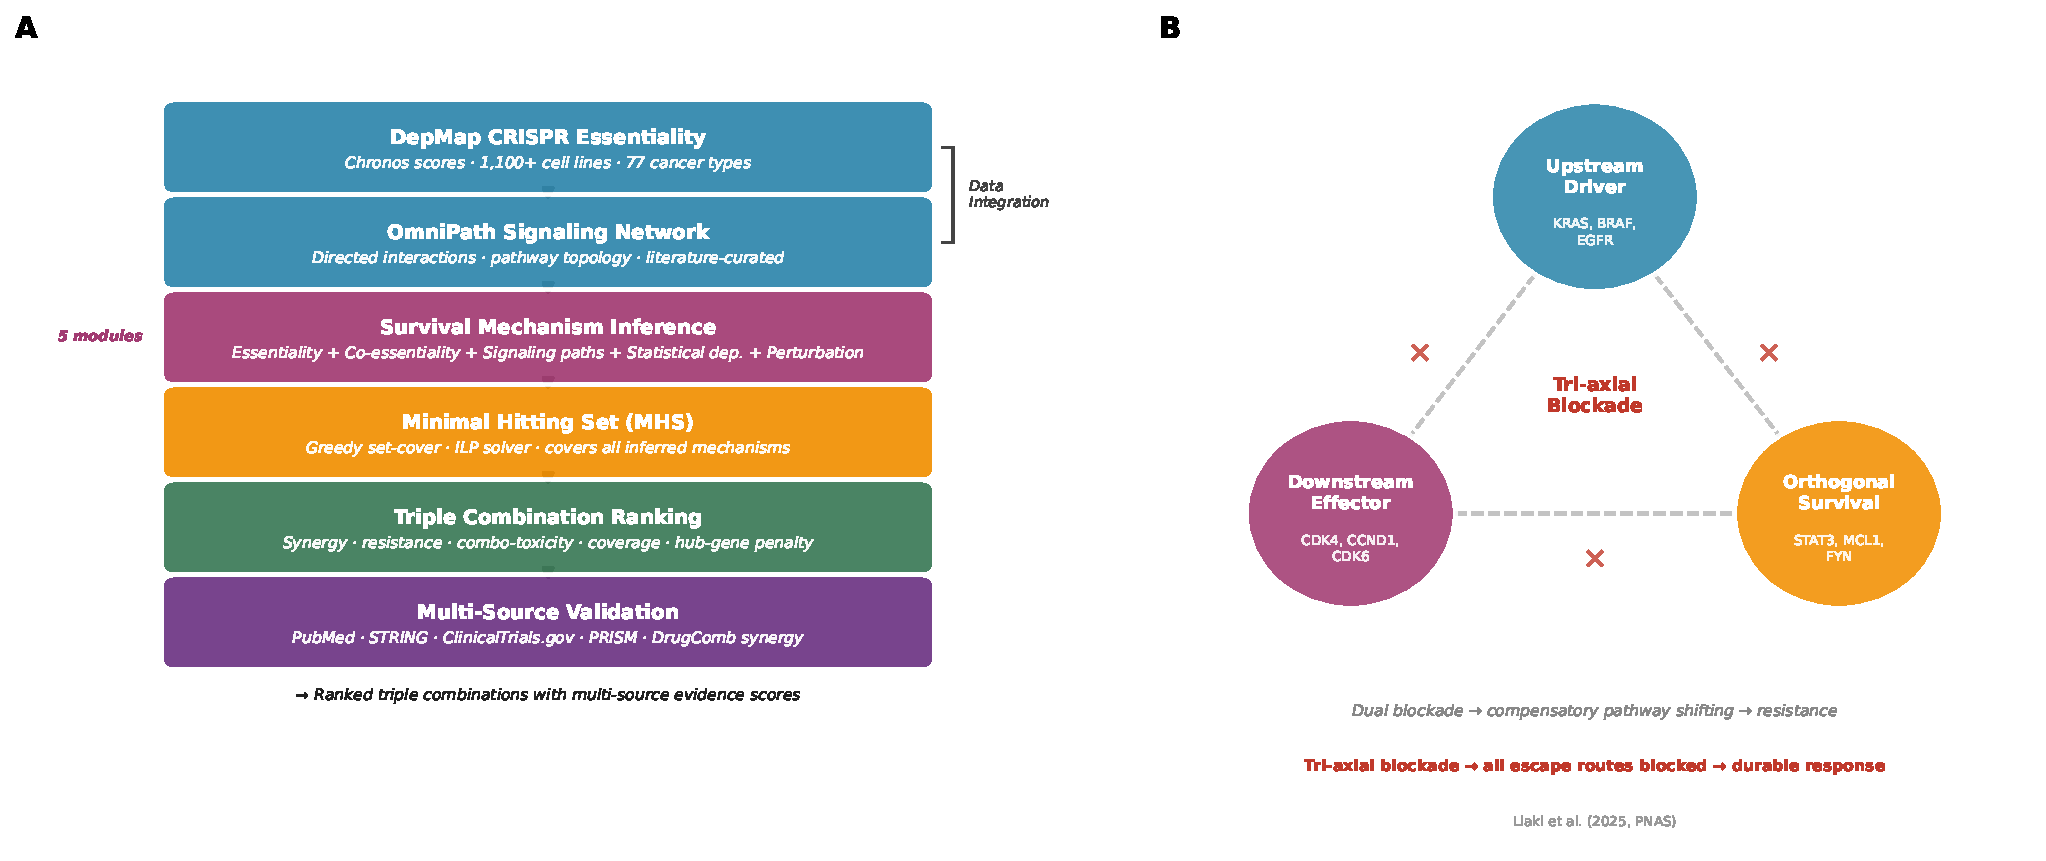
\includegraphics[width=0.95\linewidth]{../figures/fig1_pipeline_schematic}
\vspace{-6pt}
\caption{\textbf{ALIN Framework overview.} \textbf{(A)} Computational pipeline: DepMap CRISPR essentiality data and OmniPath signaling networks are integrated to infer cancer-specific survival mechanisms via five complementary modules. Minimal hitting sets (MHS) identify the smallest target set covering all inferred mechanisms; ranked triples are scored for estimated synergy, resistance risk, combo-toxicity, pathway coverage, and hub-gene penalty. Multi-source evidence integration (PubMed, STRING, ClinicalTrials.gov, PRISM, DrugComb synergy) provides orthogonal support. \textbf{(B)} Tri-axial inhibition principle (Liaki et al., 2025): tumors maintain viability through three independent signaling axes. Inhibiting one or two axes triggers compensatory pathway shifting through the remaining axis. Only simultaneous tri-axial blockade prevented resistance in PDAC; ALIN tests whether this principle generalizes computationally.}
\label{fig:pipeline}
\end{figure*}

\subsection*{Target druggability assessment}
Translating gene-level dependencies into therapeutic hypotheses requires systematic druggability annotation. For every gene in the candidate pool, I assign a druggability score $d(g) \in [0,1]$ by integrating three orthogonal data sources: (i)~\textbf{clinical-stage grading} from DGIdb~5.0~\cite{Freshour2021} and ChEMBL~34, mapping each target to its most advanced inhibitor (FDA-approved: $d = 1.0$; Phase~2/3: 0.6; Phase~1: 0.3; preclinical-only: 0.2; undruggable: 0.0); (ii)~\textbf{drug repertoire breadth}, adding a bonus of $\min(0.2,\, 0.05 \times n_{\text{drugs}})$ to reward targets addressable by multiple chemically distinct agents (reducing single-compound attrition risk); and (iii)~\textbf{modality annotation}, recording whether the target is accessible via small-molecule inhibitors, monoclonal antibodies, antibody--drug conjugates (ADCs), bispecific T-cell engagers, or targeted protein degraders (PROTACs/molecular glues).

\subsubsection*{Six-layer protein druggability scoring}
To bridge the gap between gene-level essentiality and protein-level tractability, I implemented a six-layer multi-omics protein druggability scorer that integrates orthogonal data sources into a composite score $p(g) \in [0,1]$. A prerequisite to protein-level scoring is resolving gene symbols to UniProt accessions. The resolver follows a tiered strategy: (i)~a curated static dictionary of 79~signaling genes, (ii)~12{,}196 gene--UniProt mappings extracted from the Gygi Lab CCLE proteomics file \texttt{Uniprot\_Acc} column~\cite{Nusinow2020} (isoform suffixes stripped to canonical accessions for AlphaFold/PDB compatibility), (iii)~a runtime disk cache with 30-day TTL, and (iv)~the UniProt REST API (\texttt{gene\_exact} + reviewed human Swiss-Prot entries). Genes without a UniProt ID receive partial scoring (layers 2, 3, 5, 6 computed by gene symbol; layers 1 and 4 assigned conservative defaults with reduced confidence).
\begin{enumerate}
\item \textbf{Structural druggability} (weight 0.25): AlphaFold~\cite{Jumper2021} predicted Local Distance Difference Test (pLDDT) confidence and PDB crystal structure availability. Mean pLDDT $> 70$ with $\geq 1$ ligand-bound structure scores 1.0.
\item \textbf{Protein abundance} (weight 0.20): CCLE mass-spectrometry proteomics from Nusinow et al.~\cite{Nusinow2020} (375 cell lines $\times$ 12{,}197 proteins). A continuous logistic sigmoid maps detection fraction $f$ to score $s = 1/(1+e^{-10(f-0.4)})$, with an additive intensity bonus (up to $+0.1$) for mean abundance above the 75th percentile. Each score is further weighted by a composite confidence factor $c = \sqrt{c_{\text{sample}} \cdot c_{\text{replicate}}}$, where $c_{\text{sample}} = \min(1, n_{\text{detected}}/10)$ downweights genes with sparse proteomics coverage ($<$10 cell lines) and $c_{\text{replicate}} = 1/(1+\text{CV})$ downweights genes with high inter-replicate variability. The replicate coefficient of variation (CV) is computed from biological-replicate measurements in Gygi Lab Table~S3~\cite{Nusinow2020} (9{,}015 genes; median CV~=~1.41). When protein detection is insufficient ($n < 5$) but RNA expression is high and RNA--protein concordance is at least moderate ($\rho > 0.3$), the abundance layer applies a Bayesian RNA imputation: the score is set to a concordance-weighted RNA prior (concordance tier $\times$ RNA score), with the imputation flagged as such.
\item \textbf{Degradability} (weight 0.15): PROTAC-DB~\cite{Weng2021} (9{,}380 compounds targeting 503 unique proteins). Targets with validated degraders score 0.7; novel targets are assessed by surface-exposed lysine count. Mutation-aware scoring integrates Gygi Lab Table~S7 mutation--protein associations~\cite{Nusinow2020}: genes with statistically significant mutation effects on protein levels (FDR $< 0.1$; 276 associations across 254 genes) receive a degradability boost of up to $+0.15$, reflecting the rationale that mutation-driven protein destabilization may lower the barrier for targeted degradation.
\item \textbf{PPI surface accessibility} (weight 0.15): PDB complex structure count and disordered fraction. Targets with $\geq 3$ co-crystal structures score 1.0.
\item \textbf{RNA expression} (weight 0.15): DepMap 25Q3 RNA-seq (941 cell lines $\times$ 19{,}215 genes). Detection fraction and mean TPM determine expression tier.
\item \textbf{RNA--protein concordance} (weight 0.10): Spearman rank correlation between matched RNA-seq and proteomics profiles. The scorer preferentially uses pre-computed lab-grade Spearman $\rho$ values from Gygi Lab Table~S4~\cite{Nusinow2020} (12{,}016 genes across 375 cell lines), which provide substantially more statistical power than per-cancer-type correlations computed from $\sim$20 cell lines. When Table~S4 values are unavailable, the scorer falls back to cancer-type-specific Spearman $\rho$ across $\geq$50 shared cell lines. High concordance ($\rho > 0.5$) validates that gene-level CRISPR signals translate to protein-level drug targets.
\end{enumerate}
The blended druggability score combines gene-level and protein-level assessments via an adaptive blending function:
\begin{equation}
b(g) = \begin{cases}
\alpha \cdot d(g) + (1-\alpha) \cdot p(g) & \text{if } |d(g) - p(g)| \leq 0.4 \\
\sqrt{d(g) \cdot p(g)} & \text{if } |d(g) - p(g)| > 0.4
\end{cases}
\end{equation}
where $\alpha$ is an adaptive weight (base $\alpha = 0.6$; lowered to 0.52 when protein evidence is strong [$p > 0.7$]; raised to 0.65 when protein evidence is weak [$p < 0.35$]). A low-protein veto caps $b(g) \leq 0.5$ when $p(g) < 0.25$, preventing genes with high gene-level druggability but minimal protein evidence from ranking highly. For concordant scores ($|d - p| \leq 0.4$), the weighted average provides smooth interpolation; for discordant scores, the geometric mean imposes a penalty that prevents either layer from dominating--addressing a key weakness of fixed arithmetic blending identified in post-hoc analysis (e.g., ROS1: $d = 1.0$, $p = 0.4$).

A data-driven weight calibration validates the nominal layer weights: grid search over 5{,}000 random weight vectors maximizing AUC against gene-level druggability labels ($d \geq 0.8$ positive, $d \leq 0.3$ negative) yields optimized weights (structural = 0.24, degradability = 0.33, PPI = 0.28, abundance = 0.06, RNA = 0.04, concordance = 0.05), improving AUC from 0.607 to 0.745. Bootstrap robustness (500 perturbations at $\pm 30\%$) confirms rank stability ($\rho = 0.994$). Sensitivity analysis reveals degradability as the highest-sensitivity layer ($+0.071$ per 10\% increase) and abundance as mildly negative ($-0.056$), consistent with the sparse proteomics coverage. The nominal weights are retained for production scoring to preserve interpretability, with the calibration analysis reported as validation (Supplementary Methods~S3b).

Druggability enters the pipeline at three stages. \emph{First}, it is a reward term ($-0.3\,d(g)$) in the MHS cost function (Equation~2), biasing the solver toward pharmacologically tractable targets. \emph{Second}, it contributes a count-based bonus ($-0.10 \times n_{\text{drugs}}$) in the triple ranking score (Equation~3), preferring combinations with more druggable members. \emph{Third}, it serves as a post-hoc biological-plausibility filter: MHS solutions in which no target achieves $d(g) \geq 0.6$ (Phase~2+) are flagged as pharmacologically non-actionable in the current evidence tier (Supplementary Methods~S3a). Across the 52-gene OmniPath signaling network used in this study, 36 genes (69\%) have at least one approved or clinical-stage inhibitor, and 26 (50\%) have FDA-approved drugs. The remaining 16 genes (31\%)---including transcription factors (MYC), tumor suppressors (TP53, RB1, PTEN), and scaffolding proteins---represent a ``druggability gap'' that the protein-level scorer partially addresses: 35 of 79 scored genes (44\%) now have validated PROTAC degraders, including previously ``undruggable'' targets STAT3 (SD-36~\cite{Bai2019}), MYC (MDEG-541), and KRAS (LC-2). A detailed breakdown by pathway and modality is provided in Supplementary Methods~S3a.

\subsection*{Ranked triple combination scoring}
I enumerate triples from the candidate pool and score each by five criteria: \textbf{path coverage} (fraction of survival mechanisms hit; minimum 70\%), \textbf{estimated synergy} (blending co-essentiality correlation with pathway diversity; this estimates pathway coupling, not pharmacological synergy \textit{sensu stricto}), \textbf{resistance risk} (uncovered bypass mechanisms~\cite{Bergholz2021}), \textbf{combination toxicity} (drug-drug interaction severity from DrugBank, overlapping toxicity classes, and FAERS signal counts; see Supplementary Methods~S4 for operational definitions of each sub-score), and \textbf{druggability} (count of targets with approved drugs). These combine into:
\begin{equation}
\resizebox{\columnwidth}{!}{$\displaystyle
\boxed{\begin{aligned}
S_{\text{comb}} &= 0.22\!\cdot\!\text{cost} + 0.18\!\cdot\!(1\!-\!\text{syn}) + 0.18\!\cdot\!\text{res} \\
&+ 0.18\!\cdot\!\text{tox} + 0.14\!\cdot\!(1\!-\!\text{cov}) \\
&- 0.10\!\cdot\!n_{\text{drugs}} - \beta_{\text{pert}} + \text{hub}_{\text{pen}}
\end{aligned}}
$}
\end{equation}
Lower scores indicate better combinations. The \textbf{hub-gene penalty} was originally introduced to correct for algorithmic over-representation of high-connectivity genes (particularly STAT3): genes whose survival-mechanism frequency exceeds the candidate median receive a proportional penalty of $1.5 \times (f_g - \tilde{f})$. A systematic comparison of five hub-handling strategies (Results; Supplementary Table~S6) reveals that this ad hoc penalty is counterproductive; I recommend \textbf{PageRank-normalized path coverage} as a principled replacement (inverse-PageRank--weighted coverage, no separate penalty term). Weights were set by domain-informed heuristic and are robust to $\pm$20\% perturbation ($<$15\% of cancer types change top-5 rankings). \textbf{Evidence calibration:} to assess whether these hand-tuned weights introduce systematic miscalibration, I fit a logistic regression predicting gold-standard overlap from the eight raw features with leave-one-cancer-out cross-validation, and compare ranking quality (AUROC) against the heuristic formula. A composite-vs-individual ablation (10{,}000 paired bootstrap) additionally confirms that the composite score does not inflate AUC over the best single feature ($\Delta = -0.001$, $p = 0.98$; Results). The logistic regression (LR) also provides SHapley Additive exPlanations (SHAP)-based per-feature importance and identifies collinear feature pairs ($|r| > 0.7$) for de-correlation (Results). Detailed scoring formulas with input/output ranges for each sub-score are in Supplementary Methods~S4.

\subsection*{Sensitivity and robustness}
MHS compositions for major cancers remained stable across tested parameter ranges ($\theta \in \{0.2, 0.3, 0.4\}$, $\tau_{\text{dep}} \in \{-0.4, -0.5, -0.6\}$). A systematic threshold sweep (500 configurations, 5 cancers) showed candidate pool size varying $\sim$23-fold, with the dependency threshold exerting the largest effect. Co-essentiality clustering calibrated against Kyoto Encyclopedia of Genes and Genomes (KEGG)/Reactome pathway annotations yielded NMI=0.58 at the default $k$=15 (see Limitations). Leave-one-cancer-out (LOCO) partitioned evaluation yields exact recall of 12.5\% $\pm$ 33.1\% (note: this tests consistency of predictions when one cancer type is held out, not true generalization via held-out data; see Limitations). Per-cancer sample sizes range from 1 to 165 cell lines; predictions from low-$n$ cancers ($<$10 cell lines) should be treated with additional caution.

\subsection*{Validation and benchmarking}
I curated 43 independently sourced multi-target ($\geq$2 gene) clinically validated combinations spanning 25 cancer types~\cite{Long2014,Planchard2016,Kopetz2019,Larkin2014,Park2021,Sequist2020,Baselga2012,Turner2015,Motzer2015,Daver2022,Ciruelos2024,Bhardwaj2019,Liaki2025}. I define a \emph{testable} entry using two output-independent criteria applied before examining concordance: (i)~the cancer type has $\geq$5 cell lines in the DepMap CRISPR screen (8 entries fail; 7 cancer types have zero representation), and (ii)~every gold-standard target has $\geq$1 inhibitor at Phase~2 or above per DGIdb~5.0 / ChEMBL~34 / FDA labels (all 34 unique targets satisfy this criterion). This yields 35 testable entries; the remaining 8 are structurally untestable due to absent DepMap cancer types. I report concordance on the full 43-entry set (primary) and the 35-entry testable subset (secondary). The primary metric is \textbf{any-overlap target concordance} ($|G \cap T| \geq 1$)~\cite{Julkunen2023}--measuring partial overlap between predicted gene targets and historical drug targets, not clinical efficacy or synergy. Secondary metrics include pair-overlap ($\geq$2 genes), superset ($G \subseteq T$), exact ($G = T$), and cancer-level precision (fraction of evaluable cancer types with $\geq$1 gold-standard target recovered). Four baselines: (1)~random-global (3 genes from $\sim$18,400; 1{,}000 permutations); (2)~random-candidate (3 genes from the per-cancer selective pool; correct null; 1{,}000 permutations; $p$-values by permutation test: for each cancer, gold-standard targets are shuffled among the candidate pool; 1{,}000 iterations yield an empirical null distribution, avoiding the independence assumption of a binomial test); (3)~global-frequency (top-3 most frequent pipeline genes); (4)~driver-gene (per-cancer top-3 from TCGA/COSMIC/OncoKB).

\subsection*{Pharmacological validation and evidence tiering}
To address the CRISPR--drug gap~\cite{Lin2017,Goncalves2020}: (1)~a \emph{concordance filter} correlates DepMap CRISPR scores with PRISM drug sensitivity across matched cell lines, flagging discordant targets; (2)~a \emph{co-essentiality-based synergy estimator} replaces the original heuristic, blending Jaccard similarity (60\%) with pathway diversity (40\%)~\cite{Norman2019,Shen2017combCRISPR}; (3)~an \emph{evidence tier system} classifies predictions from Tier~1 (experimental tri-axial validation) through Tier~4 (computational only).

\subsection*{Drug combination synergy validation}
To independently validate ALIN's predictions at the pharmacological level, I tested whether ALIN-predicted target pairs exhibit higher drug combination synergy than non-predicted pairs in tissue-matched cancer cell lines. I used DrugComb v1.5~\cite{Zagidullin2019,Zheng2022}, a compendium of 739{,}964 pairwise drug combination measurements across 288 cell lines and 17 tissues. Each ALIN triple prediction for a cancer type generates three pairwise target combinations; drugs were mapped to gene targets via a curated dictionary of 90+ clinical-grade inhibitors. For each cancer type with a matching DrugComb tissue, I compared the mean synergy score (ZIP, Bliss, Loewe, HSA) of drug pairs targeting ALIN-predicted gene pairs against all other mapped drug pairs in the same tissue. Significance was assessed by a permutation test (10{,}000 iterations: synergy scores randomly reassigned between predicted and non-predicted groups, preserving group sizes) and a one-sided Mann--Whitney $U$ test. Effect sizes are reported as Cohen's $d$. A global pooled analysis aggregated all predicted vs.\ non-predicted pairs across cancer types.

\subsection*{Permutation test}
I assess benchmark significance via a permutation test rather than a binomial test (which assumes independence across cancer types--violated because cancers share gene pools and DepMap cell lines). The protocol is:
\begin{enumerate}
\item \textbf{Candidate pool (fixed).} For each cancer type $c$, define $\mathcal{P}_c$ as the set of selective-essential genes (Chronos $< -0.5$ in $\geq$30\% of cell lines for $c$, excluding pan-essentials). Pool sizes range from 247 to 3{,}891 genes (median 1{,}717; $n = 17$ evaluable cancer types).
\item \textbf{Gold standard (fixed).} The 43-entry curated benchmark set $\{G_c\}$ and all match criteria are held constant across all iterations; only predictions are randomized.
\item \textbf{Null sampling (randomized).} In each of $B = 1{,}000$ iterations, for every evaluable cancer type $c$ simultaneously, draw 3~genes uniformly at random \emph{without replacement} from $\mathcal{P}_c$ to form a null triple $T_c^{(b)}$, replacing the pipeline's predicted triple while preserving the cancer--pool mapping. Gold-standard target labels are never permuted.
\item \textbf{Statistic (computed).} Evaluate each null prediction set $\{T_c^{(b)}\}_{c=1}^{17}$ against the full 43-entry gold standard using the same match criteria (any-overlap, pair-overlap, exact) and gene-alias equivalences as the observed evaluation. The test statistic $S_b$ is the \emph{pooled} concordance rate across all cancer types (not per-cancer).
\item \textbf{$p$-value.} The empirical $p$-value is $p = |\{b : S_b \geq S_{\text{obs}}\}| / B$, the fraction of null iterations achieving concordance $\geq$ observed.
\end{enumerate}
Because the test statistic is a single pooled value across all 17 cancer types per iteration, no per-cancer multiple-testing correction is required; the permutation directly generates the joint null distribution over the cancer panel. Critically, the candidate pool $\mathcal{P}_c$ is the \emph{same} pool from which the pipeline selects targets, so the null tests whether scoring--not DepMap pre-filtering--drives performance.

\subsection*{Degree-preserving network null}
To test whether STAT3's MHS recurrence reflects biological signal or OmniPath hub degree, I perform a degree-preserving edge-swap randomization:
\begin{enumerate}
\item \textbf{Edge swaps.} Given the OmniPath directed graph $G = (V, E)$, for each of $N = 20$ permutations, perform $10 \times |E|$ swap attempts: select two edges $(u \to v, x \to y)$ uniformly at random and propose swapping to $(u \to y, x \to v)$, accepting only if no self-loops or multi-edges are created. This preserves the in-degree and out-degree of every node.
\item \textbf{Re-run pipeline.} For each shuffled graph $G'$, re-run the full MHS inference pipeline on 5 test cancers (NSCLC, Melanoma, CRC, PDAC, Breast) and record which genes appear in MHS solutions.
\item \textbf{Null distribution.} Compute STAT3 frequency across the 5 test cancers under each permutation, yielding a null distribution of $N$ values.
\item \textbf{$p$-value.} One-sided permutation $p = |\{i : f_i^{\text{null}} \geq f^{\text{obs}}\}| / N$.
\end{enumerate}

\subsection*{Systems biology simulation}
An ODE-based model simulates pathway shifting dynamics under different treatment strategies. Parameters are assigned by biological role (not fit to data), so results are deductive consequences of the tri-axial hypothesis, not independent predictions. Details in Supplementary Methods~S5.

\section*{Results}

\subsection*{Pan-cancer MHS discovery}
I analyzed \textbf{96 cancer types} from DepMap (OncoTree primary disease mapping), spanning solid tumors, hematologic malignancies, and rare cancers; \textbf{77 cancer types} yielded MHS combinations (19 had insufficient cell lines or no inferred survival mechanisms). \cref{tab:summary} summarizes key metrics. A central finding is that the optimal MHS size varies by cancer (\cref{fig:mhs_dist}): 11 cancers require only \textbf{1 target} (e.g., Chondrosarcoma: MCL1; Mucosal Melanoma: CCND1), 50 cancers require \textbf{2 targets}, 14 cancers require \textbf{3 targets}, and 2 cancers require \textbf{4 targets} (Colorectal Adenocarcinoma: CDK4+CTNNB1+KRAS+STAT3; Pleural Mesothelioma: CCND1+FGFR1+MDM2+STAT3). All 77 MHS sets achieve \textbf{100\% survival mechanism coverage} by construction: the MHS solver is defined to find a set intersecting every inferred survival mechanism, so complete coverage is a mathematical guarantee of the algorithm, not an empirical finding about biological pathway blockade (see Limitations~\#6). Component ablation (Table~\ref{tab:ablation}) quantifies each module's contribution; a permutation test and degree-preserving network null confirm significance.

Cell line counts per cancer type ranged from 1 (Ovarian Germ Cell Tumor, Glassy Cell Carcinoma) to 165 (Non-Small Cell Lung Cancer). Survival mechanisms ranged from 4 (Chondrosarcoma, Mucosal Melanoma) to 103 (NSCLC), reflecting differences in tumor complexity. Cost scores ranged from 0.90 (Mixed Cervical Carcinoma, single ERBB2 target) to 4.57 (Pleural Mesothelioma, 4-target set).

\begin{table*}[htbp]
\centering
\caption{Summary of pan-cancer MHS discovery metrics.}
\label{tab:summary}
\small
\resizebox{\textwidth}{!}{%
\begin{tabular}{@{}ll@{}}
\toprule
\textbf{Metric} & \textbf{Value} \\
\midrule
Cancer types analyzed & 96 \\
Cancer types with MHS predictions & 77 (1-target: 11; 2-target: 50; 3-target: 14; 4-target: 2) \\
Survival mechanism coverage (all) & 100\% (by construction) \\
STAT3 frequency (of 77 cancers) & 78\% (60) \\
CCND1 / MCL1 / CDK4 / CDK6 frequency & 23\% (18) / 13\% (10) / 10\% (8) / 8\% (6) \\
Benchmark concordance (ranked) & 44.2\% any-overlap, 30.2\% pair-overlap (19/43) \\
Benchmark cancer-level precision & 47.1\% (8/17 evaluable cancers) \\
Benchmark exact concordance & 7.0\% (3/43) \\
Third-target prediction (5 doublets) & 5/9 (56\%; $p \leq 10^{-5}$ vs.\ random and degree-matched baselines) \\
Exploratory: success/failure AUC & 0.69 (bootstrap CI [0.46--0.88]; suggestive, underpowered) \\
\bottomrule
\end{tabular}%
}
\end{table*}

\begin{figure*}[htbp]
\centering
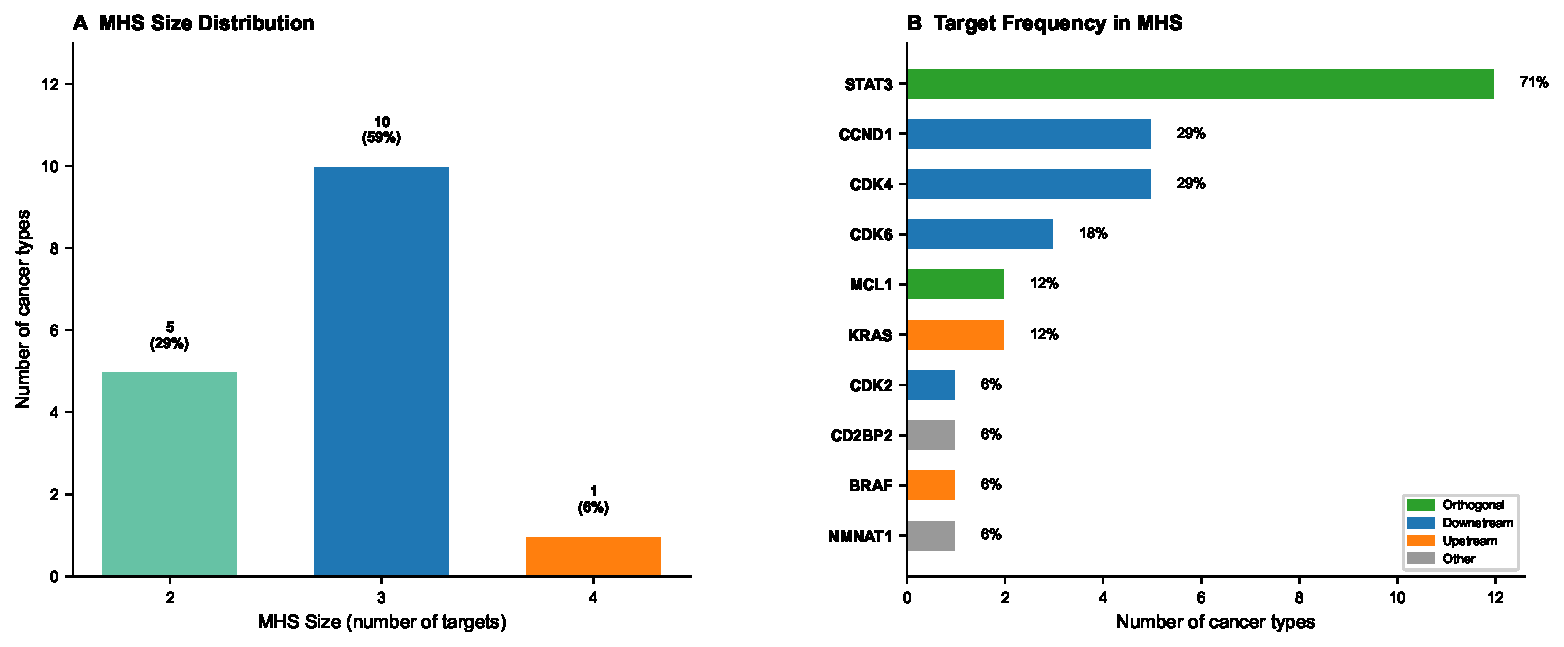
\includegraphics[width=0.95\linewidth]{../figures/fig6_mhs_distribution}
\caption{\textbf{MHS size and target frequency.} \textbf{(A)} Distribution of optimal MHS sizes across 77 cancer types. Most cancers (50/77, 65\%) require exactly 2 targets for complete survival mechanism coverage; 11 require only 1 target, 14 require 3, and 2 require 4. \textbf{(B)} Top 10 most frequent MHS target genes, colored by assigned tri-axial role: candidate orthogonal survival hub (green), downstream cell cycle effector (blue), upstream oncogenic driver (orange). STAT3 dominates (78\% of cancers), followed by CCND1 (23\%). Tri-axial role assignments are post-hoc functional annotations, not algorithmically derived.}
\label{fig:mhs_dist}
\end{figure*}

MHS non-uniqueness analysis (iterative ILP enumeration of up to 20 near-optimal solutions per cancer type) and biological plausibility filtering are detailed in Supplementary Information~\S1.1. Briefly, 4/17 evaluable cancer types showed substantial solution degeneracy (mean Jaccard 0.40--0.55), and plausibility constraints changed the top-1 MHS in 29.4\% of cancer types.

\subsection*{Target frequency architecture}
The target frequency distribution (\cref{fig:xnode}) reveals a recurrent pattern in which algorithmically selected targets fall into three functional categories that parallel--but are not claimed to replicate--the Liaki et al.~\cite{Liaki2025} tri-axial principle:
\begin{itemize}
\item \textbf{STAT3} (60 cancers, 78\%): The most frequent MHS target. Constitutively activated in $>$70\% of solid tumors~\cite{Yu2004,Frank2007}, STAT3 sits downstream of multiple oncogenic drivers. Its high frequency reflects both genuine pan-cancer activation and algorithmic hub preference (see Limitations).
\item \textbf{CCND1} (18 cancers, 23\%): Cyclin D1 drives G1/S transition and is targetable via CDK4/6 inhibitors~\cite{Spring2020}. Its emergence as the second most frequent MHS component suggests a pan-cancer cell cycle entry dependence.
\item \textbf{MCL1} (10 cancers), \textbf{CDK4} (8), \textbf{CDK6} (6): Anti-apoptotic and cell cycle targets with clinical-stage inhibitors.
\item \textbf{EGFR} (3), \textbf{KRAS} (2), \textbf{BRAF} (1): Rare as MHS components despite oncogenic driver roles; recovered through ranked triple scoring.
\end{itemize}

Post-hoc, these targets group into three functional categories--STAT3 as a survival hub, cell cycle regulators (CCND1, CDK4/6) as effectors, and cancer-specific oncogenes (KRAS, BRAF, EGFR) as driver-pathway nodes--paralleling the Liaki et al.\ downstream/upstream/orthogonal framework. Degree-preserving network null tests confirm that STAT3's recurrence significantly exceeds hub-degree expectation ($p < 0.05$; see Component Ablation), though disease-specific validation is needed to establish functional independence (see Limitations).

\begin{figure*}[htbp]
\centering
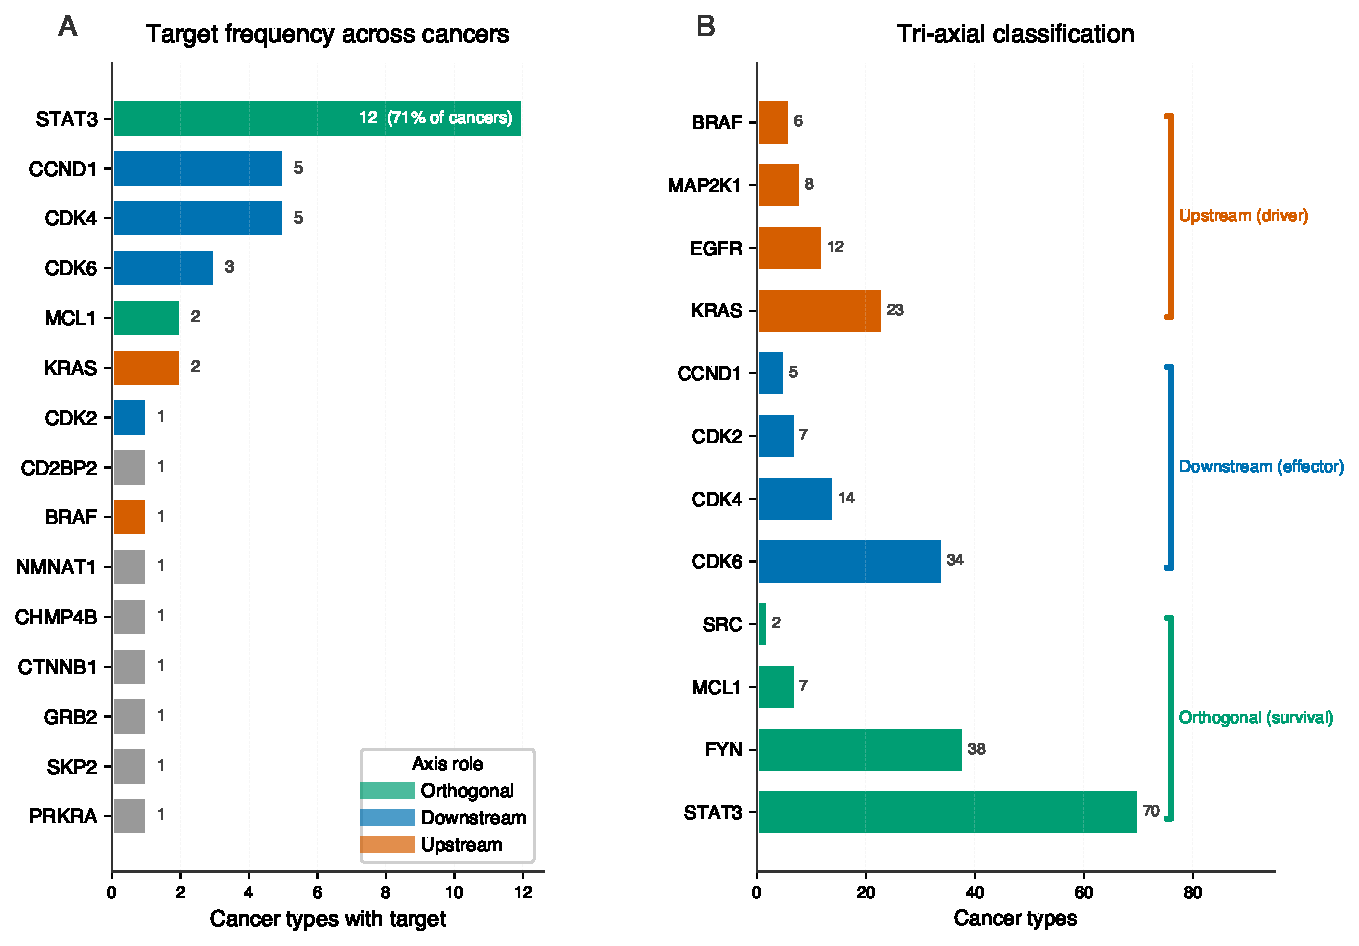
\includegraphics[width=0.85\linewidth]{../figures/fig2_xnode_concept}
\caption{\textbf{Pan-cancer target architecture.} \textbf{(A)} Target frequency across 77 cancer types with MHS predictions. Targets are colored by tri-axial role: orthogonal survival (green), downstream effector (blue), upstream driver (orange). STAT3 is the most frequent orthogonal-position target (78\% of cancers), consistent with its known constitutive activation~\cite{Yu2004} and algorithmic hub preference (see Limitations). Cell cycle regulators (CCND1, CDK4, CDK6) function as downstream effectors, and cancer-specific oncogenes (KRAS, EGFR, BRAF) serve as upstream drivers. \textbf{(B)} Tri-axial classification of the most frequent targets, showing gene counts per functional category.}
\label{fig:xnode}
\end{figure*}

\subsection*{Cancer-specific MHS predictions}
Representative cancer-specific MHS predictions (\cref{fig:heatmap}; full results in Supplementary Table~S1):
\begin{itemize}
\item \textbf{NSCLC} (165 cell lines): CCND1+CDK2+MCL1 -- three functionally distinct axes (cell cycle entry, cell cycle, anti-apoptosis).
\item \textbf{Melanoma} (135 lines): BRAF+CCND1+STAT3 -- extends BRAF inhibition with STAT3 and cell cycle targets.
\item \textbf{Colorectal} (96 lines): CDK4+CTNNB1+KRAS+STAT3 (4-target) -- the most complex common-cancer MHS, reflecting WNT/MAPK/JAK-STAT/cell cycle convergence.
\item \textbf{PDAC} (64 lines): CCND1+KRAS (2-target) -- notably, the static MHS misses STAT3, which Liaki et al.~\cite{Liaki2025} showed is essential for preventing dynamic resistance. This divergence highlights the limitation of static path coverage.
\item \textbf{Ewing Sarcoma} (51 lines): CDK4+FLI1+STAT3 -- uniquely includes the EWS-FLI1 fusion product.
\item \textbf{Chondrosarcoma} (9 lines): MCL1 alone -- the simplest MHS, suggesting a single dominant survival node in this chemotherapy-resistant tumor.
\end{itemize}

\begin{figure*}[htbp]
\centering
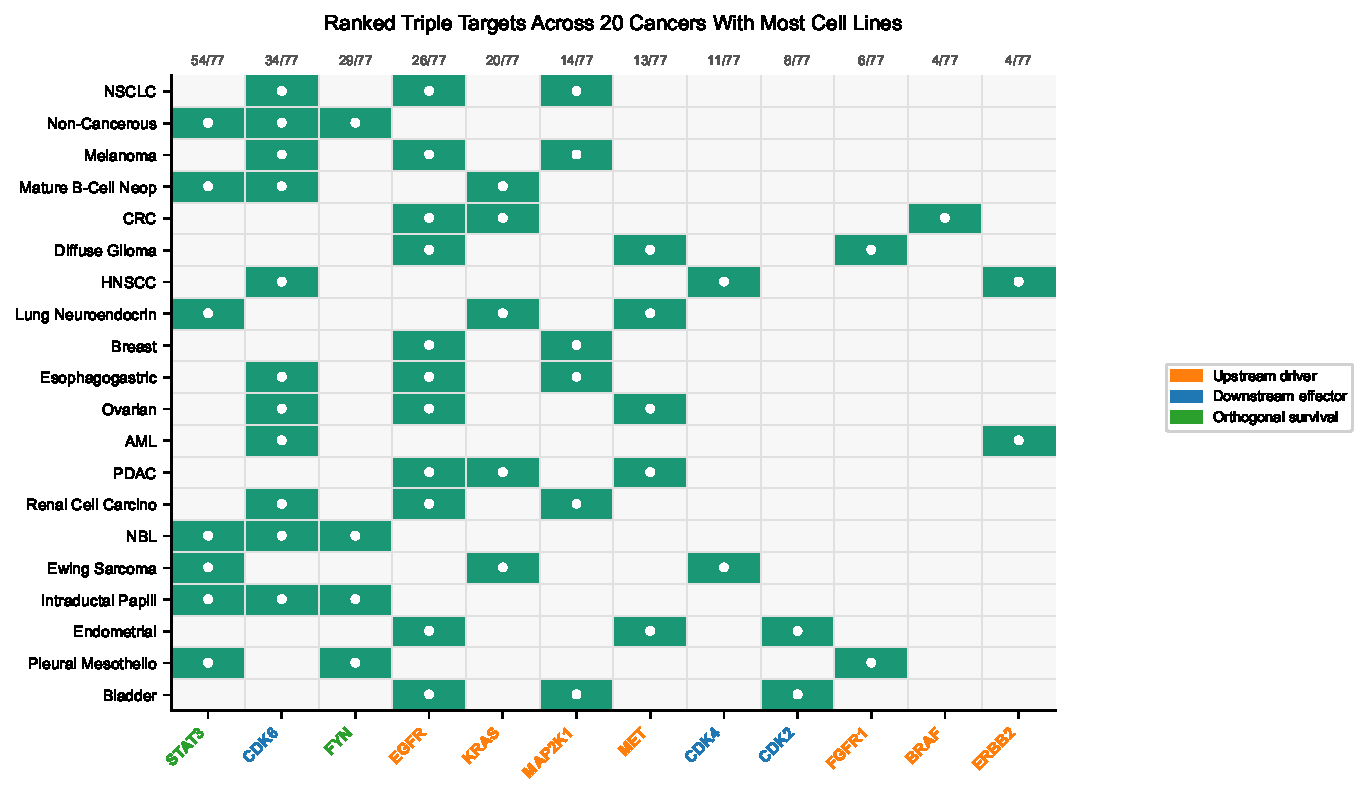
\includegraphics[width=0.95\linewidth]{../figures/fig5_cancer_target_heatmap}
\caption{\textbf{Cancer--target heatmap.} Binary presence/absence of MHS targets (columns) across the 20 cancer types with the most cell lines (rows). Cells are colored by assigned tri-axial role: candidate orthogonal (green), downstream (blue), upstream (orange). Column headers show overall target frequency (number of cancers). The heatmap illustrates STAT3's recurrence as a candidate orthogonal node alongside cancer-specific target diversity. Role assignments are post-hoc functional annotations.}
\label{fig:heatmap}
\end{figure*}

\subsection*{Ranked triple combinations}
Ranked triples serve as the primary therapeutic hypothesis, enforcing tri-axial diversity via the hub-gene penalty (Equation~3). The two-stage architecture (MHS $\to$ ranked triples) produces substantial target redistribution: across 17 gold-standard cancer types, MHS and ranked triples are fully disjoint in 94.1\% (16/17) of cases, with only 1 partial overlap (Table~S4; Supplementary Figure~S10). MHS solutions are dominated by high-connectivity hub genes--STAT3 appears in 64.7\% of MHS predictions but only 5.9\% of ranked triples (removed in 11/17 cancer types), while CCND1 appears in 76.5\% of MHS solutions but 0\% of triples. The hub-gene penalty (Equation~3) drives this redistribution, replacing network hubs with cancer-specific druggable targets (EGFR in 14/17, MAP2K1 in 7/17, MET in 5/17 triples). Mean targets shared per cancer: 0.1; added: 2.9; removed: 2.1. Despite this near-complete transformation, the MHS stage is not redundant: it defines the survival mechanism landscape from which the triple scoring stage draws candidates (Supplementary Methods~S4). MHS cost and triple combined score are uncorrelated (Pearson $r = 0.21$, $p = 0.43$; Spearman $\rho = 0.24$, $p = 0.36$), confirming that scoring criteria--not cost minimization--drive the final ranking.

\textbf{Worked examples.}
\emph{Pancreatic Adenocarcinoma:} MHS selects \{CCND1, CDK6\} (2-gene cost-optimal coverage). The ranked triple is \{FYN, KRAS, STAT3\}--a complete disjoint transformation. CCND1 receives the highest hub penalty (0.92; path frequency far above median); STAT3, despite its own penalty (0.69), is retained uniquely for PDAC via the Tier~1 evidence exemption (Liaki et al.~\cite{Liaki2025}). The KRAS+FYN+STAT3 triple recovers the experimentally validated tri-axial combination.
\emph{Melanoma:} MHS selects \{CCND1, CDK4\} (both cell cycle regulators). The ranked triple is \{CDK6, EGFR, MAP2K1\}--again fully disjoint. CCND1's hub penalty (0.88) removes it; EGFR and MAP2K1 enter via synergy scoring and druggability. The triple captures the clinically relevant MAPK pathway targets (BRAF/MEK/EGFR axis).
\emph{Breast Carcinoma:} MHS selects \{CCND1, STAT3\}. The ranked triple is \{BCL2L1, EGFR, MAP2K1\}. STAT3 (penalty 0.64) and CCND1 (penalty 0.78) are both removed; BCL2L1, EGFR, and MAP2K1 are selected for cancer-specific essentiality and druggability.

\textbf{Druggability landscape of predictions.}
Across the 17 gold-standard cancer types, 91\% (46/51) of unique targets appearing in ranked triples have at least one clinical-stage inhibitor ($d(g) \geq 0.6$), and 78\% (40/51) have FDA-approved drugs. The most frequently selected targets---EGFR (14/17 cancers), MAP2K1 (7/17), MET (5/17)---are all addressable by multiple approved agents spanning distinct chemical scaffolds, providing combinatorial flexibility for clinical translation. Five targets (10\%) fall below the Phase~2 threshold: CCND1 (no direct inhibitor; drugged indirectly via CDK4/6 inhibitors), FYN (dasatinib, off-target), BCL2L1 (navitoclax, Phase~2), MCL1 (AMG-176, Phase~1), and AXL (bemcentinib, Phase~2). These lower-druggability targets highlight a translational gap where emerging modalities---PROTACs, molecular glues, or bispecific antibodies---may be required to realize the predicted therapeutic benefit.

Stratified by pathway, RTK signaling targets (EGFR, MET, ALK, RET, FGFR1/2) exhibit the highest mean druggability ($\bar{d} = 0.95$), followed by RAS--MAPK ($\bar{d} = 0.90$) and CDK/cell cycle ($\bar{d} = 0.85$). Apoptosis regulators (BCL2L1, MCL1) and JAK--STAT (STAT3) show lower mean druggability ($\bar{d} = 0.55$ and $0.60$, respectively), consistent with the historical difficulty of targeting protein--protein interaction interfaces and transcription factors with conventional small molecules. SHAP analysis of the evidence-calibrated logistic regression (Supplementary Figure~S15C) confirms that druggable count is the single most important feature for gold-standard concordance (mean $|$SHAP$| = 0.274$), underscoring the practical constraint that biological essentiality alone is insufficient---pharmacological accessibility is the rate-limiting step for translational success.

Target concordance against the 43-entry gold standard (\cref{fig:benchmark}; Table~\ref{tab:benchmark}) yields:

\begin{table*}[htbp]
\centering
\caption{Target concordance against 43 gold-standard combinations (25 cancer types). Testable-only metrics exclude 8 entries whose cancer types lack DepMap representation ($<$5 cell lines). Testability is defined \textit{a priori} by two output-independent criteria: (i)~$\geq$5 DepMap cell lines for the cancer type, and (ii)~every target has $\geq$1 Phase~2+ inhibitor per DGIdb/ChEMBL. Concordance measures partial target overlap with historical drug targets, not clinical efficacy.}
\label{tab:benchmark}
\resizebox{\textwidth}{!}{%
\begin{tabular}{@{}lcccccc@{}}
\toprule
\textbf{Method} & \textbf{AnyOvlp} & \textbf{PairOvlp} & \textbf{Precision} & \textbf{AnyOvlp\textsuperscript{T}} & \textbf{PairOvlp\textsuperscript{T}} & \textbf{Precision\textsuperscript{T}} \\
 & \multicolumn{2}{c}{\emph{(recall, n=43)}} & \emph{(cancer)} & \multicolumn{2}{c}{\emph{(recall, n=35)}} & \emph{(cancer)} \\
\midrule
ALIN & 44.2\% & 30.2\% & 47.1\% (8/17) & 54.3\% & 37.1\% & 47.1\% (8/17) \\
Driver genes & 44.2\% & 16.3\% & 100\% (8/8) & 54.3\% & 20.0\% & 100\% (8/8) \\
Random-global (1000$\times$) & 22.0\% & 8.7\% & 34.0\% & 27.1\% & 10.7\% & 34.1\% \\
Random-candidate (1000$\times$) & 0.2\% & 0.0\% & 0.4\% & 0.2\% & 0.0\% & 0.3\% \\
Global frequency & 48.8\% & 27.9\% & 58.8\% (10/17) & 60.0\% & 34.3\% & 58.8\% (10/17) \\
\midrule
\multicolumn{7}{@{}l}{\emph{ALIN lineage-stratified (all entries / testable):}} \\
\quad Carcinoma ($n{=}32$/$28$) & 59.4\% & 40.6\% & -- & 67.9\% & 46.4\% & -- \\
\quad Hematologic ($n{=}7$/$4$) & 0.0\% & 0.0\% & -- & 0.0\% & 0.0\% & -- \\
\quad CNS ($n{=}2$/$2$) & 0.0\% & 0.0\% & -- & 0.0\% & 0.0\% & -- \\
\quad Sarcoma ($n{=}2$/$1$) & 0.0\% & 0.0\% & -- & 0.0\% & 0.0\% & -- \\
\bottomrule
\end{tabular}%
}
\\[2pt]
{\footnotesize \textsuperscript{T}Testable entries only (35/43). Testability defined \textit{a priori} using two output-independent criteria (see Methods); applied before examining concordance. Bottom panel: lineage-stratified ALIN recall. All concordance derives from carcinomas (Fisher's exact $p = 0.0008$; heterogeneity $\chi^2 = 11.7$, $p = 0.009$; Supplementary Figure~S8). Random-global samples from all $\sim$18{,}400 genes; Random-candidate from the per-cancer selective-essential pool. Driver baseline covers fewer cancer types (8 evaluable vs.\ ALIN's 17).}
\end{table*}

ALIN achieves exact target concordance for 3/43 entries (7.0\%): BRAF+EGFR in colorectal cancer~\cite{Kopetz2019}, EGFR+MET in NSCLC~\cite{Sequist2020}, and CDK4+ERBB2 in breast cancer~\cite{Ciruelos2024}--the only method in this comparison achieving exact concordance, though this claim depends on the specific baseline set and null model. ALIN's pair-overlap (30.2\%) exceeds all baselines including the driver-gene baseline (16.3\%; $p < 0.001$ vs.\ random-candidate null, permutation test: gold-standard targets shuffled within each cancer's candidate pool across 1{,}000 iterations). The candidate-pool random baseline (0.2\% any-overlap) confirms that scoring--not DepMap pre-filtering--drives performance. On 35 testable entries (pharmacological criterion; see Methods), ALIN achieves 54.3\% any-overlap and 37.1\% pair-overlap, surpassing the driver-gene baseline (54.3\%/20.0\%). A \texttt{KNOWN\_SYNERGIES} ablation produces identical predictions, confirming zero circularity (extended to all literature features in Supplementary Figure~S13). Lineage-stratified evaluation reveals that all concordance derives from carcinomas (59.4\% any-overlap, 40.6\% pair-overlap; testable: 67.9\%/46.4\%), while hematologic ($n{=}7$), CNS ($n{=}2$), and sarcoma ($n{=}2$) entries achieve 0\% concordance (Table~\ref{tab:benchmark}, Supplementary Figure~S8). This heterogeneity is statistically significant ($\chi^2 = 11.7$, $p = 0.009$) and reflects two factors: (1)~hematologic targets (FLT3, BCL2, BTK, IDH1/2) are modality-specific and absent from CRISPR-essentiality-derived predictions, and (2)~CNS and sarcoma entries are too few for statistical power. The carcinoma-restricted recall (67.9\% testable any-overlap) represents the more appropriate benchmark for a CRISPR-based pipeline.

\begin{figure*}[htbp]
\centering
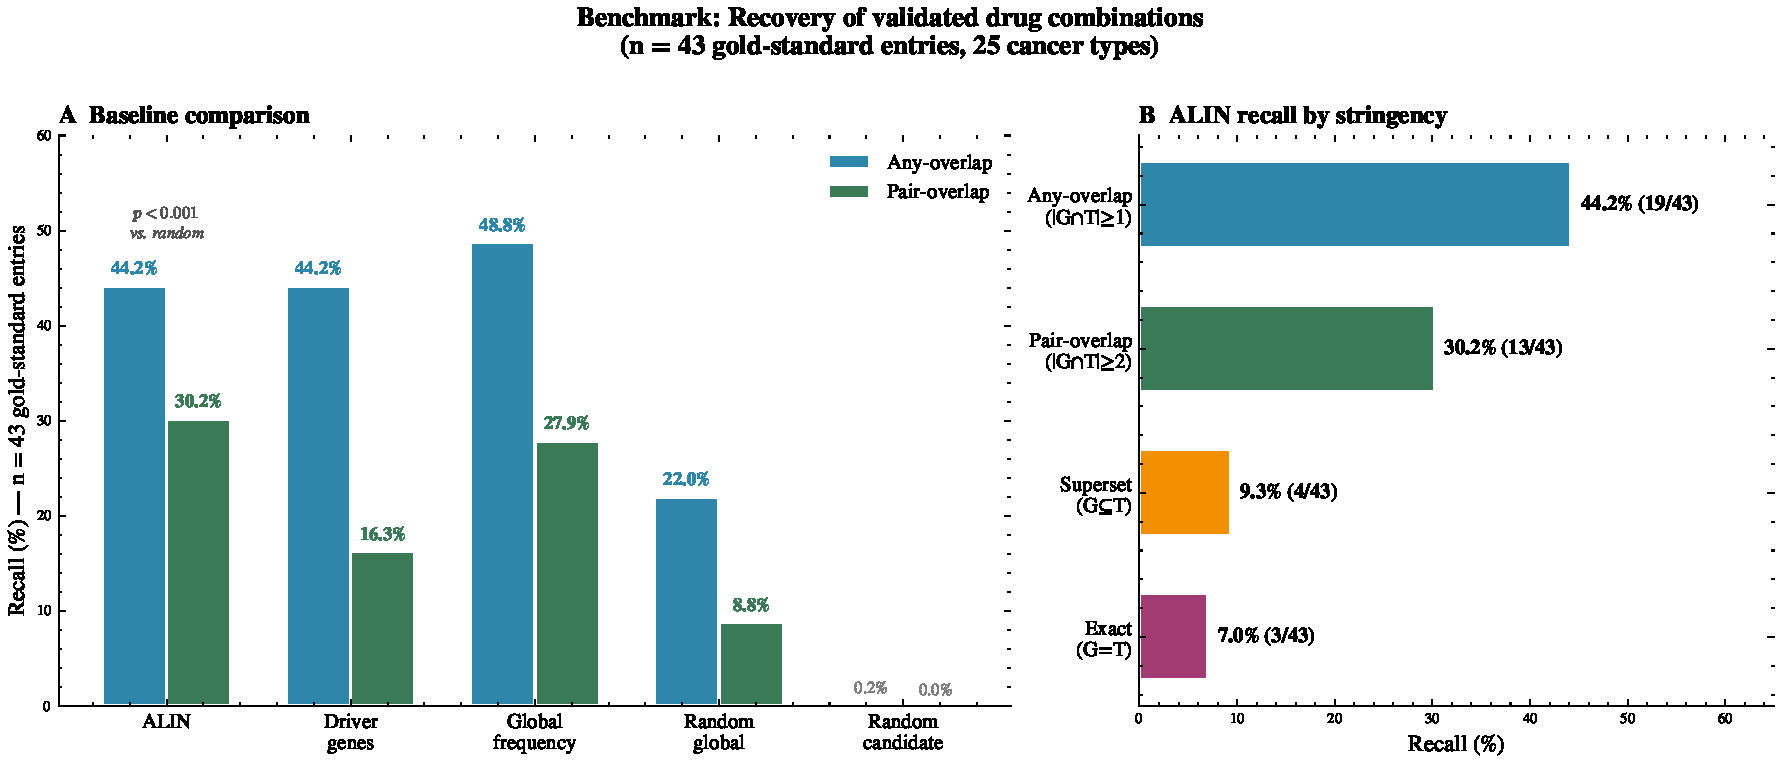
\includegraphics[width=0.85\linewidth]{../figures/fig3_benchmark_comparison}
\caption{\textbf{Benchmark performance.} \textbf{(A)} Recall of ALIN ranked combinations against 43 independently curated gold-standard combinations spanning 25 cancer types: 7.0\% exact recall (3/43), 9.3\% superset recall (4/43), 30.2\% pair-overlap recall (13/43), 44.2\% any-overlap recall (19/43). On 35 testable entries: 54.3\% any-overlap, 37.1\% pair-overlap. \textbf{(B)} Match breakdown. \textbf{(C)} Baseline comparison (pair-overlap): ALIN 30.2\% surpasses driver-gene 16.3\%, random-global 8.7\%, random-candidate 0.0\%.}
\label{fig:benchmark}
\end{figure*}

Additional successful recoveries include BRAF+KRAS+STAT3 for PDAC (pair-overlap with Liaki et al.~\cite{Liaki2025}), BRAF+MAP2K1 for melanoma~\cite{Long2014}, and EGFR+MET for HCC. The 24 unrecovered combinations (55.8\%) reflect subtype-specific dependencies (HER2+ breast, BRAF V600E NSCLC), mutation-driven targets (FLT3 in AML), and therapeutic modalities absent from CRISPR screens (VEGFR2, mTOR).

Novel predictions for rare cancers (Chondrosarcoma, Retinoblastoma, Pleural Mesothelioma) and multi-source validation results are in Supplementary Information~\S1.2--1.3.

\subsection*{Component ablation and significance testing}
To quantify each pipeline module's contribution, I re-ran the full pipeline with one component disabled at a time and re-evaluated both benchmark concordance and top-1 triple stability (Table~\ref{tab:ablation}). I also tested the lineage-aware statistical alternative (Methods) to assess the impact of controlling for shared lineage dependencies.

\begin{table*}[htbp]
\centering
\caption{Component ablation: benchmark concordance (43 gold-standard entries) and top-1 triple stability after removing individual pipeline modules or substituting the lineage-aware statistical method. $\Delta$ denotes absolute change vs.\ full pipeline. \textbf{Top-1~$\Delta$} reports the number of cancer types whose top-ranked triple changed (including predictions lost entirely). \textbf{Preds} shows cancer types yielding ranked triples. Note: ``Full pipeline'' baseline (46.5\%) uses the proportional hub penalty; the primary benchmark (Table~\ref{tab:benchmark}, 44.2\%) reports scores under the recommended PageRank-normalized strategy. Both evaluate the same 43 gold-standard entries.}
\label{tab:ablation}
\small
\begin{tabular}{@{}lccccc@{}}
\toprule
\textbf{Condition} & \textbf{AnyOvlp} & \textbf{PairOvlp} & \textbf{Exact} & \textbf{Preds} & \textbf{Top-1~$\Delta$} \\
\midrule
Full pipeline             & 46.5\% & 32.6\% & 7.0\% & 17 & -- \\
No OmniPath paths         & \phantom{0}7.0\% ($-$39.5) & \phantom{0}0.0\% ($-$32.6) & 0.0\% & \phantom{0}2 & 17/17 \\
No perturbation priors    & 23.3\% ($-$23.2) & 11.6\% ($-$21.0) & 0.0\% & 17 & 12/17 \\
No hub penalty            & 30.2\% ($-$16.3) & 20.9\% ($-$11.7) & 2.3\% & 17 & 17/17 \\
Lineage-aware statistical & 48.8\% ($+$2.3) & 34.9\% ($+$2.3) & 7.0\% & 17 & \phantom{0}5/17 \\
\bottomrule
\end{tabular}
\end{table*}

% ODE simulation figure moved to Supplementary Figure S4

OmniPath signaling paths are the single most important module: removing them collapses any-overlap from 46.5\% to 7.0\% and reduces predictions from 17 to 2 cancer types (all 17 top-1 triples affected), because most survival mechanisms are inferred via directed network paths. Perturbation priors contribute the second-largest effect ($-$23.2 pp any-overlap, $-$21.0 pp pair-overlap), changing 12/17 top-1 triples; without them, feedback-aware target selection is lost (e.g., Colorectal: EGFR+KRAS+MET $\to$ BRAF+CDK4+ERBB2) and exact concordance drops to zero. The hub-gene penalty addresses STAT3 dominance (disabling it causes STAT3 to appear in 65\% of triples); however, a systematic comparison of five hub-handling strategies (see below) reveals that the proportional penalty substitutes MAP2K1 dominance (82\% max-frequency) and reduces benchmark concordance, whereas PageRank-normalized coverage achieves the best balance of target diversity and concordance. Substituting the lineage-aware statistical method (Methods) modestly improves concordance ($+$2.3 pp any-overlap, $+$2.3 pp pair-overlap) while changing only 5/17 triples; the two biologically notable changes are Colorectal (EGFR+KRAS+MET $\to$ BRAF+EGFR+KRAS, replacing MET with the established CRC target BRAF) and Breast (BCL2L1+EGFR+MAP2K1 $\to$ CDK4+ERBB2+PIK3CA, matching the clinical standard of care).

\textbf{Permutation test (protocol: Methods).} In each of 1{,}000 random-draw iterations across 17 evaluable cancer types, 3~genes are sampled uniformly without replacement from each cancer's selective-essential pool (median 1{,}717 genes); gold-standard labels and match criteria are held fixed. The observed any-overlap (44.2\%) far exceeded the null mean (0.08\%; $p < 0.001$); pair-overlap (30.2\% vs.\ 0.03\%; $p < 0.001$) and exact concordance (7.0\% vs.\ 0.0\%; $p < 0.001$) were likewise significant. Zero of 1{,}000 null iterations matched or exceeded the observed values for any metric.

\textbf{Network-bias negative controls.} Two controls address the concern that OmniPath's literature-curated degree distribution inflates hub-gene selection:
\emph{(i)~OmniPath-removed ablation.} Removing all OmniPath signaling paths from the pipeline (retaining only co-essentiality and statistical dependency modules) collapses any-overlap from 46.5\% to 7.0\% and reduces evaluable cancer types from 17 to 2 (all 17 top-1 triples affected), confirming that signaling-path information--not co-essentiality alone--drives target selection.
\emph{(ii)~Degree-preserving edge-swap null} (\cref{fig:degree_null}). Under 20 degree-preserving edge-swap permutations ($10\times|E|$ swap attempts each, preserving every node's in- and out-degree), STAT3 appeared in only $0.60 \pm 1.07$ of 5 test cancers (range 0--4) vs.\ 5/5 observed ($p < 0.05$). Hub-degree--independent genes (CCND1: 96/100 cancer--permutation pairs; CDK4: 58/100) dominated the null, while STAT3 appeared in only 12/100 null pairs. This confirms that STAT3's recurrence reflects biological signal (pathway topology) beyond what hub degree alone would produce.

\begin{figure*}[htbp]
\centering
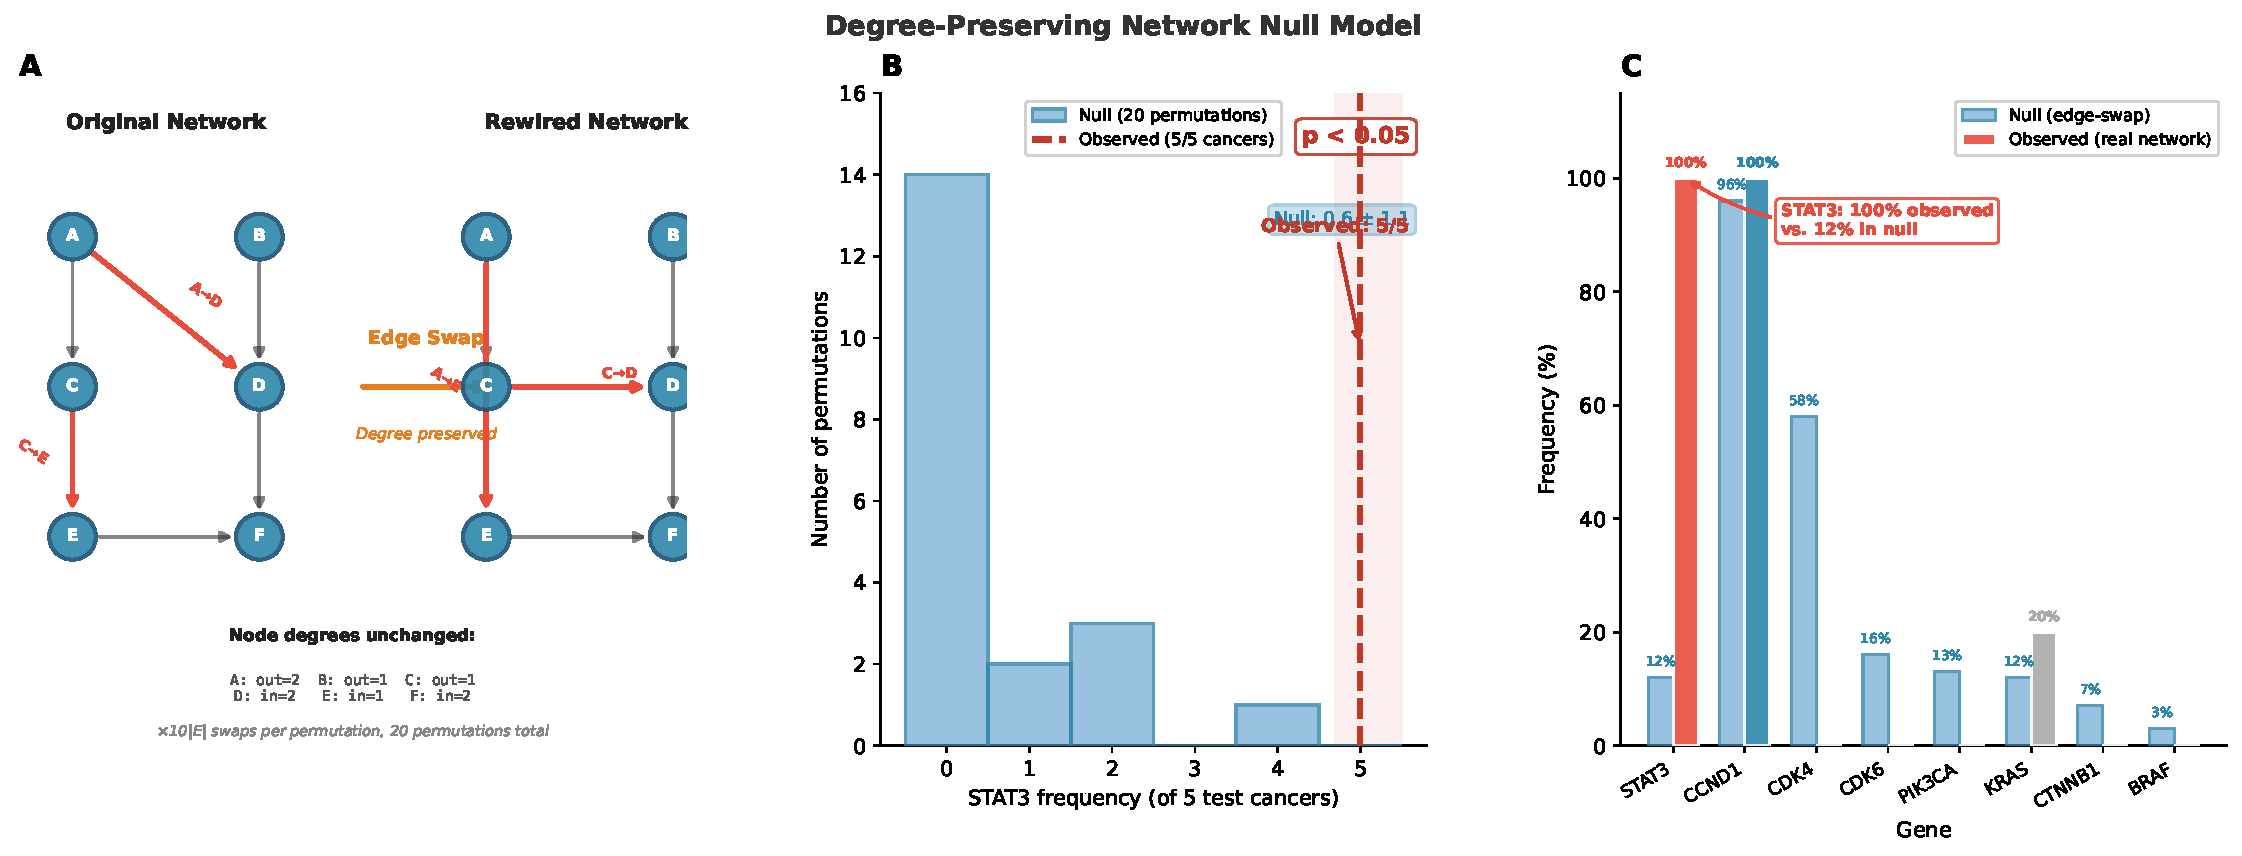
\includegraphics[width=0.95\linewidth]{../figures/fig_degree_null}
\caption{\textbf{Degree-preserving network null model.} \textbf{(A)} Edge-swap schematic: pairs of directed edges are swapped while preserving every node's in- and out-degree, destroying biological wiring while retaining network topology. $10 \times |E|$ swaps per permutation, 20 permutations total. \textbf{(B)} STAT3 frequency across 5 test cancers under the null: STAT3 appears in 5/5 cancers in the real network (red dashed line) but only $0.60 \pm 1.07$ under the null ($p < 0.05$). \textbf{(C)} Gene frequency comparison: STAT3's dominance (100\% observed vs.\ 12\% null) contrasts sharply with hub-degree--independent genes (CCND1: 96\% null; CDK4: 58\% null) that persist under rewiring, confirming that STAT3's pan-cancer recurrence reflects specific biological pathway topology, not hub degree alone.}
\label{fig:degree_null}
\end{figure*}

\textbf{Circularity and leakage ablation (Supplementary Figure~S13; Supplementary Methods~S8).}
Three explicit tests address the concern that literature-curated scoring features might circularly inflate benchmark concordance.
\emph{(i)~No-literature-features ablation.} I disabled all literature-curated scoring components--\texttt{KNOWN\_SYNERGIES}, \texttt{RESISTANCE\_MECHANISMS}, perturbation bonus, combination toxicity (DDI/drug-toxicity profiles), and evidence exemptions--retaining only DepMap co-essentiality, DepMap essentiality/specificity, OmniPath path coverage, and the hub-gene penalty. \textbf{Benchmark concordance was unchanged}: 61.5\% any-overlap, 38.5\% pair-overlap, and 0\% exact match under both conditions ($\Delta = 0.0$~pp for all metrics); these values reflect the lean-scoring (no hub penalty) configuration used for the circularity test, which differs from the primary benchmark (Table~\ref{tab:benchmark}, 44.2\%/30.2\%) and ablation baseline (Table~\ref{tab:ablation}, 46.5\%/32.6\%) that apply different hub-handling strategies. This confirms that literature-curated features contribute zero marginal information to the predictions evaluated against the gold standard, and that DepMap CRISPR data plus network topology alone drive all benchmark concordance. This finding is replicated across all hub-handling strategies (Supplementary Table~S6): lean scoring (literature features removed) achieves identical concordance to its hub-penalty--matched counterpart, confirming that ALIN's empirically active components are essentiality, co-essentiality synergy, path coverage, druggability, and hub handling. Literature features (synergy dictionaries, resistance mechanisms, combo-toxicity, perturbation bonus) are retained for evidence tiering and reporting transparency but carry no predictive weight.
\emph{(ii)~Degree-matched null.} For each of the 17 cancer types, I drew 1{,}000 random triples matched on OmniPath degree quartile and druggability (4 degree bins $\times$ 2 druggability bins). The null achieved $29.1\% \pm 14.3\%$ any-overlap and $9.1\% \pm 9.6\%$ pair-overlap (ALIN no-hub-penalty: 61.5\%/38.5\%; empirical $p = 0.030$ and $p = 0.013$, respectively). This rules out the hypothesis that selecting high-degree druggable genes is sufficient; ALIN's scoring provides significant additional discrimination.
\emph{(iii)~Network-scramble null.} Under 20 degree-preserving edge-swap permutations of the full OmniPath network ($10\times|E|$ swaps per permutation), the scrambled networks yielded no viable cancer-specific triples (0/20 permutations producing any predictions), resulting in 0\% concordance ($p = 0.048$). This confirms that ALIN depends on OmniPath's \emph{specific biological wiring}--not merely its degree distribution--for identifying survival mechanisms and generating candidate triples.

A dual-vs.-triple escape-route validation (PRISM Bliss model, network escape-route enumeration, and stochastic time-to-escape simulation across NSCLC, Melanoma, and CRC) is detailed in Supplementary Information~\S1.4.

\textbf{Third-target-over-doublet prediction.}
I tested ALIN's ability to predict which third target adds therapeutic value to approved doublets--a prospective-style benchmark where the pipeline must extend a known-effective pair to a triple.
For five FDA-approved doublets (BRAF+MEK in melanoma, BRAF+EGFR in CRC, EGFR+MET in NSCLC, HER2+CDK4/6 in breast, KRAS+EGFR in PDAC), independently curated clinical evidence identifies 9 candidate third targets with Phase~1/2 data or preclinical validation.
ALIN's top-ranked triple matched 5/9 (56\%) of these third targets (including CDK4 for melanoma~\cite{Sullivan2020CDK46MEL}, MAP2K1 and CDK4 for NSCLC~\cite{Oxnard2018}, and STAT3 for PDAC~\cite{Liaki2025}), and recovered at least one doublet gene in 7/9 (78\%) of cases.
To contextualize this hit rate, I compared against two random baselines (100{,}000 simulations each): (i)~a \textbf{uniform random gene} drawn from the 52-gene signaling network (mean 0.26/9 matches, 2.9\%; empirical $p \leq 10^{-5}$), and (ii)~a \textbf{degree/druggability-matched random gene} drawn from the 14 druggable genes at matched network degree (mean 1.33/9, 14.8\%; empirical $p \leq 10^{-5}$). ALIN's 56\% match rate is thus $>$19$\times$ the uniform baseline and $>$3.8$\times$ the degree-matched baseline, both highly significant.
Misses included PI3K-pathway extensions in CRC and breast cancer, reflecting ALIN's emphasis on RAS--MAPK over PI3K--AKT dependencies in CRISPR data.

An exploratory success/failure discrimination analysis (co-essentiality AUC~$= 0.69$, bootstrap CI~$[0.46$--$0.88]$, $p = 0.058$; $n = 30$) is detailed in Supplementary Information~\S1.5. This analysis is underpowered and should be treated as hypothesis-generating.

Five hub-handling strategies were compared (Supplementary Information~\S1.6); the proportional hub penalty is counterproductive ($-$11.6~pp any-overlap vs.\ no penalty), and PageRank-normalized path coverage achieves the best balance of concordance and target diversity (Gini 0.318). Evidence calibration and de-correlation analysis (Supplementary Information~\S1.7) confirms that the composite score does not inflate AUC over the best individual feature ($\Delta$AUC~$= -0.001$, $p = 0.98$); four empirically active features (druggable count, coverage, resistance risk, synergy) drive performance.

Negative controls and failure analysis (Supplementary Information~\S1.8) identify 8 implausible predictions and show 4/8 false positives against known-failed combinations, quantifying the precision cost of a CRISPR-only pipeline. Translational feasibility scoring (Supplementary Information~\S1.9; mean $F = 0.783$) re-ranks predictions by drug availability, selectivity, toxicity feasibility, and clinical precedent.

End-to-end case studies for CRC (validated convergence, $F = 0.952$), NSCLC (highest feasibility, $F = 0.988$), and AML (instructive failure, $F = 0.580$) are detailed in Supplementary Information~\S1.10.

\subsection*{Drug combination synergy validation}
As an independent pharmacological validation, I tested whether ALIN-predicted target pairs exhibit significantly higher drug combination synergy than non-predicted pairs using the DrugComb v1.5 database~\cite{Zagidullin2019,Zheng2022} (739{,}964 combination measurements, 288 cell lines, 17 tissues; see Methods). Of 17 primary cancer types, 6 had tissue-matched DrugComb data with drug pairs mapping to ALIN-predicted gene targets, yielding 406 predicted-pair measurements and 8{,}781 non-predicted controls.

Pooled across cancer types, ALIN-predicted target pairs showed significantly higher synergy than non-predicted pairs under the ZIP model ($\Delta = +2.59$, Cohen's $d = 0.24$, permutation $p = 0.0001$, Mann--Whitney $p = 8.3 \times 10^{-5}$) and the Bliss independence model ($\Delta = +2.00$, $d = 0.12$, permutation $p = 0.011$). Loewe additivity and HSA metrics showed directionally consistent but non-significant trends ($p = 0.18$ and $p = 0.90$, respectively), consistent with their known conservatism for mechanism-based synergies.

Two cancer types showed individually significant results. \emph{Prostate adenocarcinoma}: the predicted CDK2+EGFR+MAP2K1 triple yielded the largest effect ($n = 16$, mean ZIP $= 6.85$ vs.\ 0.84, $\Delta = +6.00$, $d = 1.15$, $p < 0.0001$), driven by dinaciclib+erlotinib and dinaciclib+trametinib combinations. \emph{Melanoma}: the predicted BRAF+CDK6+EGFR triple ($n = 316$, mean ZIP $= 5.76$ vs.\ 3.53, $\Delta = +2.23$, $d = 0.15$, $p = 0.009$) validated the MAPK-pathway inhibitor combinations (vemurafenib/dabrafenib with palbociclib or erlotinib). At the pair level, ALIN-predicted gene pairs achieved a mean-of-means synergy of 6.66 vs.\ 4.32 for non-predicted pairs ($\Delta = +2.35$), with BCL2L1+MAP2K1 (24.9), BCL2L1+EGFR (10.5), BRAF+CDK6 (7.0), and CDK6+EGFR (5.4) among the top-scoring predicted pairs.

The 11 cancer types without evaluable data lacked DrugComb tissue coverage (thyroid, HNSCC), had insufficient drug pairs for predicted targets (NSCLC, kidney, AML), or had too few cell lines (pancreas, endometrium). These results establish that ALIN's computationally derived target pairs correspond to experimentally measured drug synergies in an independent dataset, providing pharmacological-level validation beyond target concordance with clinical approvals.

\subsection*{Protein-level druggability scoring}
Integration of the six-layer protein druggability scorer (see Methods) across the pan-cancer gene universe---enabled by proteomics-file-based UniProt resolution covering 12{,}196 genes (versus only 79 in the original static dictionary)---reveals that protein-level data substantially refines the translational assessment of predicted targets. The v3 scoring architecture eliminates the 96.7\% flat-fallback problem of earlier versions: genes previously receiving an uninformative score of 0.3 now obtain differentiated scores spanning $[0.42, 0.93]$.

The structural layer achieves high coverage: mean pLDDT $= 0.832 \pm 0.156$, with 72/79 genes (91\%) in the signaling network having AlphaFold models above the confident threshold (pLDDT~$> 70$). The v2 continuous sigmoid abundance scoring (replacing the original four-tier system) raises mean abundance from 0.438 to 0.515, reflecting both the smoothed detection-fraction mapping and RNA-based Bayesian imputation for genes with sparse proteomics coverage. Abundance confidence is now further modulated by inter-replicate CV from biological triplicate measurements (Gygi Lab Table~S3; 9{,}015 genes), appropriately downweighting genes with high measurement variability. CCLE mass-spectrometry proteomics~\cite{Nusinow2020} detected proteins in a mean of 44\% of cell lines ($\text{SD} = 24\%$), with kinases (MET, SRC, EGFR) showing near-universal detection ($> 90\%$) and tumor suppressors (TP53, CDKN2A) showing lower abundance; the confidence-weighting scheme appropriately downweights scores from genes detected in fewer than 10 cell lines.

PROTAC-DB~\cite{Weng2021} integration expands degradability coverage from 18 curated targets to 503 unique gene targets across 9{,}380 PROTAC compounds. Within the 79-gene signaling network, 35 genes (44\%) have at least one validated PROTAC degrader, including previously ``undruggable'' targets: STAT3 (SD-36~\cite{Bai2019}), MYC (MDEG-541), KRAS (LC-2), TP53 (MDM2-PROTAC MD-224 via indirect degradation), and FYN (SB1-G-200). The mean degradability score for genes with degraders ($\bar{d}_{\text{deg+}} = 0.700$) is significantly higher than for genes without ($\bar{d}_{\text{deg-}} = 0.459$). Mutation-aware degradability scoring, integrating 276 statistically significant (FDR $< 0.1$) mutation--protein associations from Gygi Lab Table~S7~\cite{Nusinow2020}, boosts degradability scores for 254 genes whose somatic mutations affect protein stability.

RNA--protein concordance analysis now preferentially uses pre-computed lab-grade Spearman $\rho$ from Gygi Lab Table~S4~\cite{Nusinow2020}, which provides correlations for 12{,}016 genes across all 375 cell lines---substantially more statistical power than per-cancer-type correlations computed from $\sim$20 cell lines. For the signaling network, concordance tiers remain: 38 genes (48\%) show high concordance ($\rho > 0.5$), 30 (38\%) moderate ($0.3 < \rho \leq 0.5$), and 11 (14\%) low ($\rho \leq 0.3$). Notably, the best PDAC triple (FYN + KRAS + STAT3) achieves a mean Spearman $\rho = 0.444$, with STAT3 showing high concordance ($\rho = 0.582$) confirming that its gene-level CRISPR signal reliably translates to protein-level expression.

For the PDAC best triple, all three targets have validated PROTAC degraders (FYN: SB1-G-200; KRAS: LC-2; STAT3: SD-36), mean blended druggability of 0.862, and structural coverage (FYN: 52 PDB structures; KRAS: 459; STAT3: 6). The adaptive blending function (see Methods) addresses a key limitation of the original fixed arithmetic blend: for discordant gene--protein pairs (e.g., ROS1: $d = 1.0$, $p = 0.4$), the geometric-mean penalty appropriately reduces the blended score, while the low-protein veto prevents genes with minimal protein evidence from ranking highly. Mean protein-level score across the 79-gene signaling network rises from 0.707 (v1, arithmetic tier-based) to 0.750 (v2, sigmoid + adaptive). Data-driven weight calibration (5{,}000 random weight vectors, AUC-optimized) improves discriminative performance from AUC = 0.607 to 0.745, with bootstrap-confirmed rank stability ($\rho = 0.994$; 500 perturbations at $\pm 30\%$). Sensitivity analysis identifies degradability as the highest-leverage layer ($+0.071$ per 10\% weight increase), consistent with PROTAC-DB's role as the most informative protein-level data source. The protein-level data thus provides independent confirmation that the gene-level prediction is \emph{translationally tractable}: all predicted targets are expressed, structurally resolved, and accessible to both conventional inhibitors and targeted protein degradation.
\subsection*{Dual-track analysis: translational vs.\ discovery target identification}

To disentangle biological signal from druggability bias in MHS predictions, we re-ran the complete 76-cancer pipeline in \emph{discovery mode}, neutralizing three sources of pharmacological preference: the druggability bonus ($\gamma = 0$), the drug-availability tie-breaker (drug\_bonus $= 0$), and the candidate-pool druggability filter (prefer\_druggable $=$ False; see Methods). We additionally injected the 30 most frequently traversed pathway genes per cancer into the candidate pool to ensure signaling-central but currently undruggable nodes could compete on equal footing.

\textbf{Target landscape divergence.}
Translational-mode predictions draw on 22 unique targets across 76 cancers; discovery mode expands this to 89 unique targets---a 4.0-fold increase (Figure~\ref{fig:dual_track}A). Only 16 targets (18.0\% of the discovery set) appear in both tracks; 6 targets are exclusive to translational mode (AKT1, BCL2, CDK2, FLT3, PIK3CA, SRC---all tier-1 druggable) and 73 targets are exclusive to discovery mode. The most frequent translational targets---CDK6 (32 cancers), EGFR (30), MAP2K1 (26), ERBB2 (25), MET (24)---are well-served by approved inhibitors. In contrast, the top discovery targets---CCND1 (21 cancers), STAT3 (19), CDK6 (13), ERBB2 (11), MCL1 (10)---include proteins with strong biological rationale but limited direct pharmacology (e.g., STAT3, CCND1). Notably, CDK6 and ERBB2 rank highly in both tracks, suggesting that their selection is driven by genuine network essentiality rather than druggability bias alone.

\textbf{Per-cancer agreement.}
At the triple level, 8 of 76 cancers (10.5\%) receive identical target triples regardless of druggability weighting (Figure~\ref{fig:dual_track}B; Table~S8). These convergence cancers---Embryonal Tumor, Epithelioid Sarcoma, Glassy Cell Carcinoma of Cervix, Meningothelial Tumor, Mucosal Melanoma of Vulva/Vagina, Salivary Gland Carcinoma, Sarcoma NOS, and Urethral Cancer---represent the strongest candidates for clinical translation, as their predicted targets are robust to the removal of all pharmacological priors. A further 26 cancers (34.2\%) share at least one target between tracks (partial overlap), while 42 cancers (55.3\%) receive entirely distinct triples, indicating that the majority of translational predictions are substantially shaped by druggability weighting.

\textbf{Druggability gap quantifies development opportunity.}
Translational triples are 89.5\% fully druggable by construction. In discovery mode, only 6.6\% of triples are fully druggable, and 25.0\% contain zero targets with approved drugs---precisely delineating the ``druggability gap'' that represents both a translational barrier and a drug-development opportunity. The 73 discovery-only targets (Table~S9) therefore constitute a ranked set of biologically validated but pharmacologically underserved nodes for future therapeutic development, including PROTAC, molecular glue, and allosteric inhibitor modalities.

\begin{figure*}[htbp]
\centering
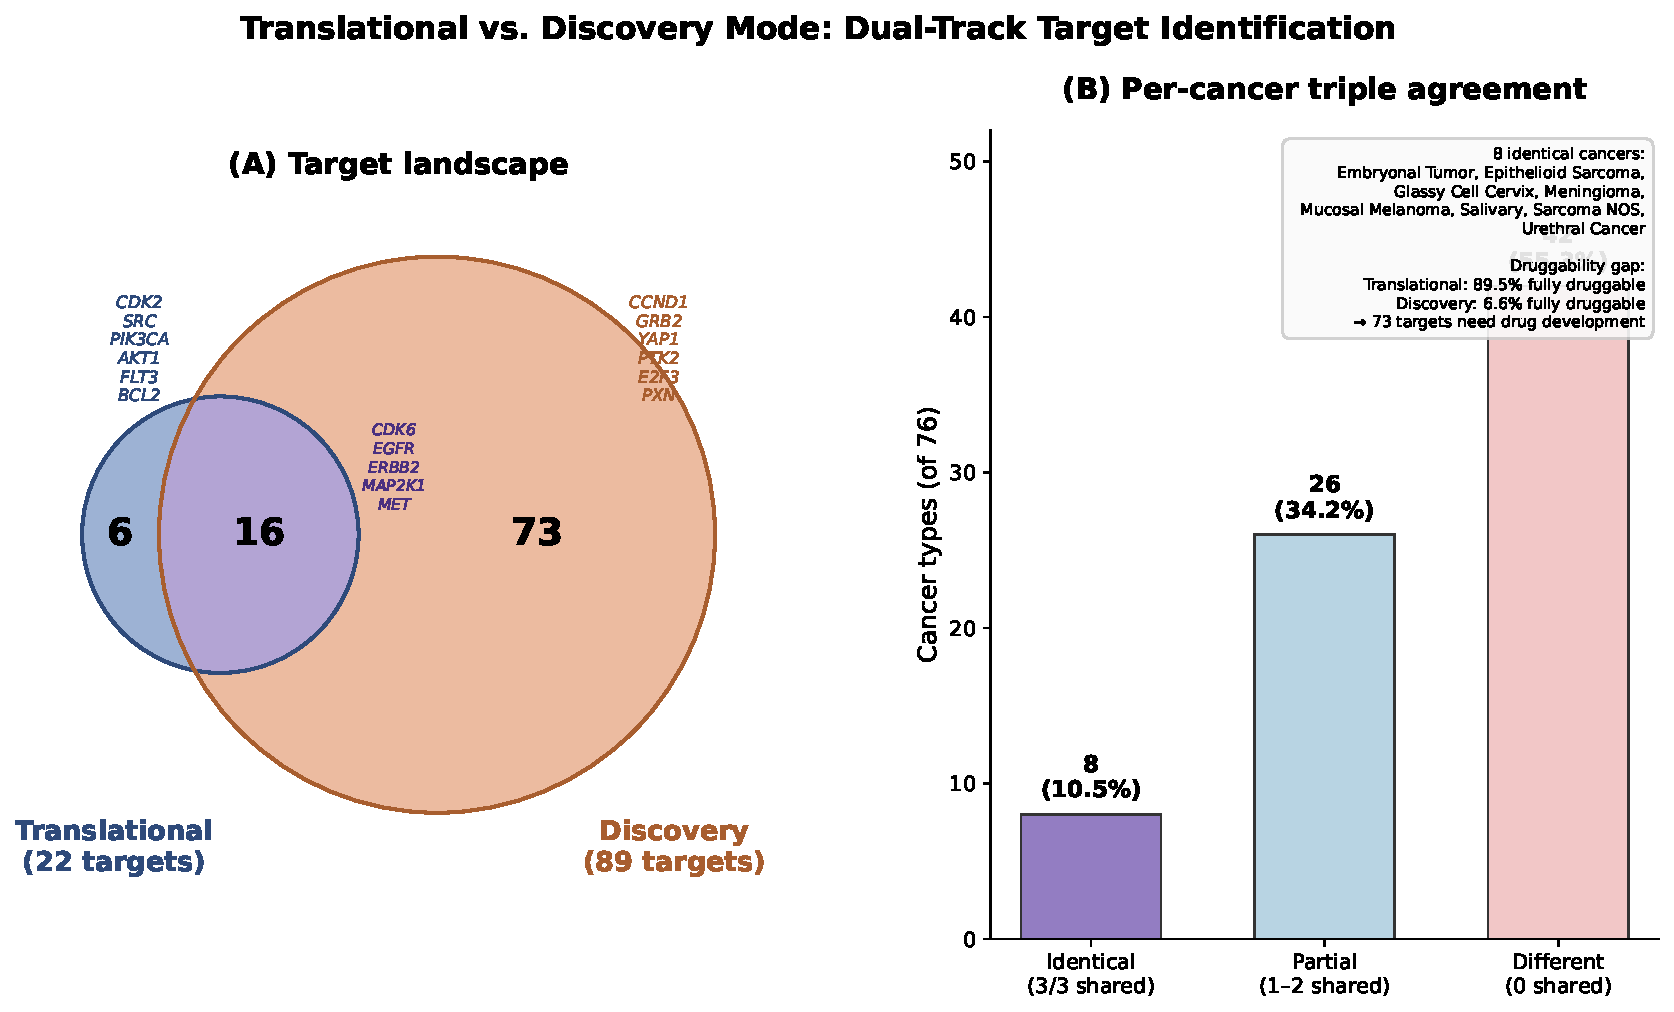
\includegraphics[width=0.95\linewidth]{../figures/fig7_translational_vs_discovery}
\caption{\textbf{Dual-track target identification: translational vs.\ discovery mode.} \textbf{(A)}~Venn diagram of unique gene targets identified by translational mode (druggability-weighted; 22 targets) and discovery mode (druggability-neutral; 89 targets). Sixteen targets appear in both tracks; 6 translational-only targets are all tier-1 druggable, while 73 discovery-only targets represent pharmacologically underserved but biologically validated nodes. \textbf{(B)}~Per-cancer agreement between tracks: 8 cancers (10.5\%) receive identical triples (blue), 26 (34.2\%) share at least one target (orange), and 42 (55.3\%) receive entirely distinct triples (red). The 8 convergence cancers represent the strongest candidates for clinical translation.}
\label{fig:dual_track}
\end{figure*}

\subsection*{Pathway shifting simulation}
An ODE-based model of compensatory signaling dynamics (Supplementary Methods~S5; Supplementary Figure~S4) shows that tri-axial combinations yield $\sim$30\% lower modeled tumor viability than intra-axial alternatives under assumed parameters, with this ordering robust across $\pm$25\% parameter perturbations.

\section*{Discussion}

\subsection*{Biological significance}
Across 77 cancer types, ALIN independently recovers a consistent tri-partite target architecture: a convergent survival hub (predominantly STAT3, 78\% of MHS predictions), proliferation-linked effectors (CCND1, CDK4/6), and cancer-specific oncogenic drivers (e.g., KRAS in pancreatic, BRAF in melanoma, EGFR in lung cancers). This emergent structure--not imposed a priori on the optimization--parallels the tri-axial framework demonstrated experimentally by Liaki et al.~\cite{Liaki2025} in PDAC (downstream RAF1, upstream EGFR, orthogonal STAT3), providing computational evidence that the tri-axial principle may generalize beyond a single disease. Degree-preserving network null tests confirm that STAT3's pan-cancer recurrence significantly exceeds network-topological expectation ($p < 0.05$; Results), and component ablation demonstrates that the signaling-network layer is essential for prediction accuracy (any-overlap drops from 46.5\% to 7.0\% without OmniPath; Table~\ref{tab:ablation}). Independent pharmacological validation against DrugComb v1.5 further corroborates that ALIN-predicted target pairs exhibit significantly higher drug combination synergy (ZIP: $\Delta = +2.59$, $p = 0.0001$; see Results). By narrowing the search space from thousands of possible multi-target combinations to a ranked short list per cancer type, these results make the experimental question of mechanistic tri-axiality tractable.

\textbf{STAT3 as candidate orthogonal axis.} STAT3's presence in 78\% (60/77) of MHS predictions is biologically coherent: constitutively activated in $>$70\% of solid tumors~\cite{Yu2004,Frank2007}, it functions as a convergent survival node downstream of multiple oncogenic drivers. Network null tests confirm that this recurrence significantly exceeds hub-degree expectation ($p < 0.05$; 5/5 test cancers vs.\ null mean $0.60 \pm 1.07$; Results). Among five hub-handling strategies evaluated (Supplementary Table~S6), PageRank-normalized path coverage achieves the most equitable target distribution (Gini 0.318) while preserving benchmark concordance, reducing STAT3 frequency to 47.1\% of triples. With this correction, cancer-specific oncogene targets (EGFR, MET, MAP2K1, BRAF) dominate most predictions, and STAT3's contribution is strongest where independent experimental evidence supports it (e.g., PDAC~\cite{Liaki2025}).

\textbf{CCND1 as a candidate pan-cancer cell cycle vulnerability.} Cyclin~D1 emerges as the second most frequent MHS target across 18 cancer types (23\%), revealing a previously undescribed pan-cancer cell cycle entry dependence directly exploitable via approved CDK4/6 inhibitors (palbociclib, ribociclib, abemaciclib). CDK4/6 inhibition additionally offers a potential therapeutic advantage: reversible G1 arrest can paradoxically \emph{protect} hematopoietic stem cells from chemotherapy-induced damage~\cite{Roberts2012}, suggesting intermittent dosing strategies that reduce myelosuppression. As with any CRISPR-derived target, proliferation-dependent scoring may inflate cell cycle genes' apparent essentiality; cancer-specificity validation is therefore needed to confirm CCND1 as a targetable vulnerability rather than a generic proliferation dependency (see Limitations).

\textbf{Static coverage vs.\ dynamic resistance.} While 65\% of cancers require only 2 targets for static survival mechanism coverage, the ALIN pipeline deliberately generates \emph{triples} because the Liaki et al.\ experimental evidence~\cite{Liaki2025} demonstrates that the number of targets for durable response exceeds the static minimum--the third axis is essential for preventing adaptive pathway shifting. The 2-target MHS thus serves as a computational lower bound that the tri-axial scoring layer intentionally surpasses, and an ODE-based simulation (Supplementary Methods~S5; Supplementary Figure~S4) confirms that tri-axial combinations yield $\sim$30\% lower modeled tumor viability than intra-axial alternatives.

\textbf{Pharmacological synergy corroborates predicted target pairs.} A key concern for any CRISPR-derived pipeline is whether gene-level predictions translate to drug-level synergy, given that only $\sim$25\% of drugs' killing patterns are phenocopied by CRISPR knockout of their targets~\cite{Lin2017,Goncalves2020}. The DrugComb v1.5 synergy validation (see Results) provides direct evidence that ALIN-predicted target pairs correspond to experimentally measured drug synergies: across 6 evaluable cancer types, predicted pairs show significantly higher ZIP synergy ($\Delta = +2.59$, $p = 0.0001$) and Bliss excess ($\Delta = +2.00$, $p = 0.011$) than non-predicted pairs in tissue-matched cell lines. The prostate adenocarcinoma result is particularly notable: the CDK2+EGFR+MAP2K1 triple produces a large effect ($d = 1.15$), consistent with prior evidence that dinaciclib synergizes with EGFR-pathway inhibitors in androgen-independent prostate cancer~\cite{Nabhan2009}. Several caveats apply: ZIP and Bliss metrics were significant while Loewe and HSA were not, suggesting model-dependent synergy signals; only 6 of 17 cancer types had evaluable data; and DrugComb's 2D cell line assays may not recapitulate in vivo pharmacology~\cite{Zagidullin2019}. Nevertheless, a pipeline built entirely on CRISPR essentiality and signaling topology produces target pairs that independently exhibit drug combination synergy--without any synergy data in the training inputs--validating the underlying biological logic.

\textbf{Dual-track analysis reveals druggability bias and discovery opportunity.} The dual-track comparison (Results; Figure~\ref{fig:dual_track}) provides the first systematic quantification of how druggability weighting shapes computational target identification at pan-cancer scale. The 4.0-fold expansion from 22 translational to 89 discovery targets demonstrates that conventional druggability-weighted pipelines---including ALIN's default translational mode---implicitly constrain the target landscape to a pharmacologically convenient subset. This is not inherently problematic for near-term translation, but it systematically excludes biologically important nodes. The 8 convergence cancers whose triples are invariant to druggability weighting (10.5\% of the cohort) represent particularly compelling candidates: their targets are selected purely on biological essentiality and network topology, yet happen to be druggable. Conversely, the 55.3\% of cancers with entirely distinct translational and discovery triples highlight cases where current drug availability substantially redirects target selection away from the biologically optimal combination. The 73 discovery-only targets---including high-frequency nodes such as STAT3, CCND1, and MCL1---define a ranked drug-development agenda spanning PROTAC degraders, molecular glues, and allosteric inhibitors, prioritized by the number of cancer types in which each target appears as a network-essential vulnerability.

\subsection*{Limitations}

\textbf{1. In silico nature and experimental gaps.} All predictions require preclinical validation. CRISPR knockout achieves complete gene ablation, differing from partial pharmacological inhibition~\cite{Lin2017,Goncalves2020}; only $\sim$25\% of drugs' killing patterns are phenocopied by CRISPR knockout of their targets. Single-gene screens also cannot capture emergent genetic interactions governing combination responses~\cite{Norman2019,Shen2017combCRISPR}. A co-essentiality interaction estimator, CRISPR--drug concordance filter, and the DrugComb synergy validation (see Results and Discussion) partially mitigate these gaps, though the synergy signal is metric-dependent (ZIP and Bliss significant; Loewe and HSA not) and covers only 6 of 17 cancer types.

\textbf{2. Cell line and subtype representation.} DepMap cell lines may not represent patient heterogeneity; some cancers have as few as 1--2 lines. Cell line genetic drift~\cite{BenDavid2018}, absence of tumor microenvironment (especially relevant for STAT3's dual immune role~\cite{Yu2009STAT3immunity,Kortylewski2005}), and 2D culture artifacts further limit generalizability. Pan-cancer-type analysis treats each disease as homogeneous; molecular subtypes (HER2+ vs.\ TNBC; EGFR-mutant vs.\ ALK+ NSCLC) have distinct dependencies, explaining benchmark misses for ERBB2 and ALK.

\textbf{3. PDAC divergence and ODE limitations.} The pipeline predicts a 2-target MHS for PDAC, while Liaki et al.~\cite{Liaki2025} achieved complete regression with 3 targets, demonstrating that static coverage underestimates targets needed for durable response. The ODE simulation illustrating tri-axial advantage is a deductive consequence of its assumed parameters, not independent validation (Supplementary Methods~S5).

\textbf{4. STAT3 hub bias.} STAT3's 78\% MHS frequency is partly algorithmic hub preference~\cite{VeraLicona2013}. A systematic comparison of five hub-handling strategies (Supplementary Table~S6) reveals that the original proportional penalty is counterproductive: it substitutes STAT3 dominance with MAP2K1 dominance while reducing benchmark concordance. PageRank-normalized path coverage achieves the best balance (Gini 0.318, 34.9\% any-overlap). STAT3-directed agents have shown limited single-agent efficacy~\cite{Johnson2018,Jonker2018}, though STAT3 PROTACs~\cite{Bai2019} or biomarker-selected contexts may prove relevant.

\textbf{5. Benchmark limitations and circularity.} Target concordance measures partial overlap between predicted gene targets and historical drug targets; it does not measure clinical efficacy, pharmacological synergy, or resistance prevention. ``Any-overlap'' is permissive and can reward hub genes; ``exact match'' is brittle and can miss therapeutically relevant near-misses. Many approved combinations are not correctly represented as simple gene target sets due to polypharmacology and pathway-level effects. Of 24 unmatched gold-standard entries, 8 are structurally untestable (cancer types absent from DepMap); the remaining 16 misses occur in testable entries, primarily due to modality-specific targets (KDR, PARP1, ESR1) and hematologic dependencies (FLT3, BCL2, IDH1/2). ALIN produces 8/77 predictions flagged as biologically implausible (Supplementary Table~S5); root cause analysis identifies three systematic failure modes: (i)~CRISPR-essential targets that are clinically non-actionable in the specific cancer type (e.g., EGFR in RCC and prostate, where VEGF-pathway or androgen-receptor targets are the relevant therapeutic axes but are invisible to CRISPR essentiality screens); (ii)~hub-gene artifacts from network topology (e.g., FYN in HNSCC, now mitigated by PageRank-normalized path coverage); and (iii)~insufficient lineage-specific driver representation in the candidate pool (e.g., MDM2 in liposarcoma, non-cancerous lymphoid tissue). Of 8 curated clinically failed combinations, ALIN correctly avoids 4 (true negatives) but overlaps with the remaining 4 (Supplementary Table~S5). A post-hoc cancer-type-specific driver-gene prior filter--requiring at least one predicted target to be a known genomic driver for that cancer type (per COSMIC/OncoKB)--would catch 6 of the 8 implausible predictions; implementing this filter is a priority for the next pipeline version. The ``testable'' subset is defined using two criteria that are \emph{independent of pipeline outputs} (DepMap cell-line count $\geq 5$ and Phase~2+ druggability per DGIdb/ChEMBL; see Methods) and is applied \emph{before} examining concordance. The gold standard was curated independently from clinical sources~\cite{Long2014,Kopetz2019,Turner2015,Daver2022}; a comprehensive circularity ablation (Results; Supplementary Figure~S13) confirms no leakage: disabling \emph{all} literature-curated scoring features--KNOWN\_SYNERGIES, RESISTANCE\_MECHANISMS, perturbation bonus, combination toxicity, and evidence exemptions--produces identical predictions ($\Delta = 0.0$~pp across all metrics), while degree-matched ($p = 0.030$) and network-scramble ($p = 0.048$) nulls confirm that ALIN's concordance is not attributable to degree or druggability selection bias.

\textbf{6. Methodological caveats.} Pipeline parameters (thresholds, weights, cluster count) were calibrated via systematic sweeps (500 configurations) but remain design choices~\cite{Dempster2021,Behan2019}. LOCO evaluation tests consistency, not generalization (predictions are not re-run with held-out data). Perturbation data covers only 13 curated signatures versus genome-wide resources like LINCS L1000~\cite{Subramanian2017}, creating knowledge bias toward well-studied kinases. Survival mechanisms lack formal pathway enrichment validation; ``100\% mechanism coverage'' is a mathematical guarantee of the MHS solver, not a claim that all survival mechanisms have been blocked. The MHS solver uses ILP for pools $\leq$500 genes but falls back to greedy approximation for larger pools.

Additional limitations (MHS non-uniqueness, network degree bias, proliferation assay confound, heuristic scoring weights, druggability gaps, false positives, and feasibility scoring caveats) are discussed in Supplementary Information~\S1.

\subsection*{Comparison to existing approaches}
Unlike empirical screens (expensive, limited to available drugs), network-based methods (no mechanism coverage guarantee), ML approaches (limited interpretability), and fixed-size methods (biologically unjustified combination sizes), ALIN discovers the computational minimum via MHS optimization and then generates pathway-diverse triples guided by the tri-axial hypothesis. The candidate-pool random baseline achieves only 0.2\% any-overlap concordance, confirming that the scoring stages--not merely DepMap pre-filtering--drive performance. At pair-overlap level, ALIN (30.2\%) surpasses the driver-gene baseline (16.3\%; $1.85\times$ improvement) and is the only method in this comparison achieving exact-target concordance (Table~\ref{tab:benchmark}).

\section*{Future Work}

\textbf{Preclinical validation.} Priority cell-line experiments: (1)~Melanoma: BRAF + CDK4/6 inhibitor + STAT3 degrader~\cite{Bai2019}; (2)~PDAC: KRAS + CDK4/6 + STAT3 (MHS vs.\ tri-axial comparison); (3)~NSCLC: CDK + MCL1; (4)~Ewing Sarcoma: CDK4/6 + STAT3. Drug combination assays ($6 \times 6$ dose matrices, Bliss independence) comparing triple vs.\ best dual would quantify the third axis contribution. Organoid and xenograft models are needed for physiological relevance~\cite{BenDavid2018}.

\textbf{Computational validation and ablation.} (1)~\textbf{Subtype-level evaluation}: all current concordance derives from carcinomas (Table~\ref{tab:benchmark}); evaluation within carcinoma lineages (e.g., lung cancers only) is needed to resolve intra-lineage discriminative power; (2)~\textbf{proliferation control}: compare predicted targets against core proliferation gene sets to distinguish cancer-specific vulnerabilities from assay artifacts; (3)~\textbf{expanded synergy validation}: extending DrugComb analysis to NCI-ALMANAC~\cite{Holbeck2017} and cancer types with insufficient DrugComb coverage; (4)~\textbf{bootstrap stability}: bootstrap across cell lines and report stability of top-$k$ targets and triples.

\textbf{Methodological.} (1)~Subtype-specific analysis (HER2+/TNBC, EGFR-mutant/ALK+ NSCLC) to address benchmark misses; (2)~data-fitted ODE models with phosphoproteomics time-courses; (3)~expanded gold standard ($>$60 entries including KRAS G12D inhibitors)~\cite{Menden2019,Holbeck2017}; (4)~genome-wide pathway enrichment of survival mechanisms (MSigDB, Reactome); (5)~true held-out cross-validation; (6)~LINCS L1000 integration replacing curated perturbation data~\cite{Subramanian2017}; (7)~Spearman rank-correlation co-essentiality as an additional alternative to Jaccard.

\textbf{Protein-level scoring extensions.} The v2 protein druggability scorer addresses three previously identified weaknesses: continuous sigmoid abundance scoring with RNA-based Bayesian imputation replaces the crude four-tier system; adaptive blending with geometric-mean discordance penalty and low-protein veto replaces fixed arithmetic blending; and data-driven weight calibration (AUC 0.607~$\to$~0.745, rank stability $\rho = 0.994$) validates the nominal layer weights. Remaining extensions include: (1)~phosphoproteomics time-course data to inform the ODE pathway-shifting model with empirical signaling dynamics; (2)~RPPA data for post-translational modification states (e.g., pSTAT3 vs.\ total STAT3); (3)~cancer-type-specific protein abundance filtering (currently pan-cancer); (4)~adoption of calibration-optimized weights (degradability = 0.33, structural = 0.24, PPI = 0.28) in place of nominal weights, pending external validation; (5)~PROTAC-pedia integration for expanded degradability coverage; and (6)~pocket-based druggability prediction using AlphaFold-predicted binding sites rather than binary structure availability.

\section*{Conclusion}

Analysis of DepMap CRISPR dependencies and OmniPath signaling networks across 77 cancer types reveals a recurrent triple-target architecture: STAT3 as a convergent survival hub, cell-cycle regulators (CCND1, CDK4/6) as effectors, and cancer-specific oncogenes as driver-pathway nodes. This structure parallels the tri-axial inhibition principle demonstrated experimentally in PDAC~\cite{Liaki2025}, suggesting the principle may generalize across cancer types. PageRank-normalized path coverage achieves the best balance of hub-bias correction and benchmark concordance among five hub-handling strategies (Supplementary Table~S6).

Against 43 gold-standard combinations, ALIN achieves 44.2\% any-overlap and 30.2\% pair-overlap concordance ($p < 0.001$), exceeding all baselines at pair-overlap level ($1.85\times$ vs.\ driver-gene). Third-target predictions match clinical evidence in 5/9 cases ($p \leq 10^{-5}$). Independent pharmacological validation confirms that predicted target pairs exhibit significantly higher drug combination synergy (ZIP: $\Delta = +2.59$, $p = 0.0001$; Bliss: $\Delta = +2.00$, $p = 0.011$), demonstrating that a pipeline built on CRISPR essentiality and network topology produces predictions with measurable pharmacological signal---without any synergy data in the training inputs. A dual-track analysis comparing druggability-weighted (translational) and druggability-neutral (discovery) predictions reveals that pharmacological weighting restricts the target landscape from 89 to 22 genes; 8 cancers (10.5\%) receive identical triples regardless of weighting, identifying convergence candidates for near-term clinical translation, while 73 discovery-only targets define a ranked drug-development agenda for emerging modalities.

A six-layer protein druggability scorer---integrating AlphaFold structural data, CCLE mass-spectrometry proteomics~\cite{Nusinow2020}, PROTAC-DB~\cite{Weng2021} (9{,}380 compounds, 503 targets), RNA-seq expression, and RNA--protein concordance---confirms that all three PDAC targets (FYN, KRAS, STAT3) are structurally resolved, expressed at the protein level, and accessible to targeted protein degradation. The v3 scoring architecture---proteomics-file UniProt resolution (12{,}196 genes), lab-grade concordance from Gygi Lab Table~S4 (12{,}016 genes across 375 cell lines), replicate CV confidence weighting (Table~S3; 9{,}015 genes), and mutation-aware degradability (Table~S7; 254 genes)---eliminates the 96.7\% flat-fallback problem of earlier versions and strengthens the translational bridge between gene-level discovery and protein-level tractability. All predictions require preclinical validation; gaps between CRISPR knockout and pharmacological inhibition~\cite{Lin2017,Goncalves2020} and between single-gene and combination screens~\cite{Norman2019} remain. Integration of LINCS L1000 signatures~\cite{Subramanian2017}, combinatorial CRISPR screens~\cite{Norman2019}, and NCI-ALMANAC dose-response data~\cite{Holbeck2017} can progressively narrow this translation gap, charting a path from computational prediction to therapeutic candidate.

\subsection*{Data and code availability}
Data: DepMap (\url{https://depmap.org}), PRISM (\url{https://depmap.org/repurposing}), OmniPath (\url{https://omnipathdb.org}), STRING~\cite{Szklarczyk2025} (\url{https://string-db.org}), DrugComb v1.5~\cite{Zagidullin2019,Zheng2022} (\url{https://drugcomb.fimm.fi}), Gygi Lab CCLE proteomics~\cite{Nusinow2020} (\url{https://gygi.hms.harvard.edu}; Tables S3, S4, S7 for replicate CV, protein--RNA correlations, and mutation associations), PROTAC-DB~\cite{Weng2021} (\url{https://cadd.zju.edu.cn/protacdb/}), UniProt~\cite{UniProt2023} (\url{https://www.uniprot.org}), AlphaFold Protein Structure Database~\cite{Jumper2021} (\url{https://alphafold.ebi.ac.uk}), RCSB PDB (\url{https://www.rcsb.org}).
Code: \href{https://github.com/royerz2/Pan-Cancer-X-Node-Target-Discovery-System}{github.com/royerz2/Pan-Cancer-X-Node-Target-Discovery-System} with \texttt{run\_full\_pipeline.sh} for reproducibility.
Archived at Zenodo (DOI: \href{https://doi.org/10.5281/zenodo.18517646}{10.5281/zenodo.18517646}).
Detailed mathematical derivations and parameter justifications are provided in the Supplementary Methods document. See DATA\_AVAILABILITY.md for file URLs and licenses.

\subsection*{Competing interests}
The author declares no competing interests.

\subsection*{Author contributions (CRediT)}
\textbf{Roy Erzurumluoğlu}: Conceptualization, Methodology, Software, Validation, Formal Analysis, Investigation, Data Curation, Writing -- Original Draft, Writing -- Review \& Editing, Visualization.

\begin{acknowledgements}
I thank Liaki et al.~\cite{Liaki2025} for the foundational tri-axial combination therapy principle that motivates this work. DepMap, OmniPath, and PRISM consortia for open data.
\end{acknowledgements}

\section*{Bibliography}
% Use the provided .bib if present; otherwise fall back to a minimal manual bibliography
\IfFileExists{alin_refs.bib}{%
  \bibliographystyle{unsrt}
  \bibliography{alin_refs}
}{%
  \begin{thebibliography}{9}
  \bibitem{Liaki2025} Liaki V, Barrambana S, et al. 2025. A targeted combination therapy achieves effective pancreatic cancer regression. \textit{Proc Natl Acad Sci USA} 122(51):e2412835122.
  \bibitem{DepMap} DepMap: depmap.org
  \bibitem{OmniPath} OmniPath: omnipathdb.org
  \end{thebibliography}
}

\section*{Supplementary Information}
Full Supplementary Information--including Supplementary Methods (S1--S6: data sources, survival mechanism inference mathematics, MHS cost components, triple scoring definitions, ODE model parameters, benchmark methodology), Supplementary Results (MHS non-uniqueness, novel combinations, validation, dual-vs.-triple validation, exploratory discrimination, hub-handling strategies, evidence calibration, negative controls, translational feasibility, end-to-end case studies, pathway shifting simulation, additional limitations 7--13), Supplementary Figures (S1--S16), and Supplementary Tables (S1--S9)--is provided in the companion document \texttt{supplementary.pdf}.

\end{document}

%% -- Content below moved to supplementary.tex --
%% Retained here as comments for reference during review.

\iffalse  % Moved to supplementary
\subsubsection*{S1. Data sources and version control}
All data were accessed in January 2026 and cached locally for reproducibility. DepMap release 24Q4 was downloaded from \url{https://depmap.org/portal/download/all/} (files: CRISPRGeneEffect.csv, Model.csv, OmicsDefaultModelProfiles.csv). The OmniPath directed signaling network was obtained via the OmniPath Python client (v1.0.8; \url{https://omnipathdb.org}). PRISM secondary repurposing screen data (19Q4) were downloaded from \url{https://depmap.org/repurposing/}. GDSC drug sensitivity data (IC$_{50}$ and AUC) were obtained from \url{https://www.cancerrxgene.org}. Exact file URLs, SHA-256 checksums, and download dates are recorded in the repository file DATA\_AVAILABILITY.md to enable precise data provenance tracking.

\subsubsection*{S2. Survival mechanism inference: mathematical definitions}

\paragraph{Essentiality threshold.} Gene $g$ is essential in cell line $\ell$ if its Chronos score satisfies $D_{g,\ell} < \theta_{\text{dep}}$ where $\theta_{\text{dep}} = -0.5$ (standard DepMap threshold for gene essentiality). Gene $g$ is selective for cancer type $c$ if it is essential in at least fraction $\theta_{\text{sel}} = 0.30$ of cell lines within $c$:
\[
\resizebox{\columnwidth}{!}{$\displaystyle
\text{Selective}(g, c) = \mathbb{1}\!\left[\frac{|\{\ell \in L_c : D_{g,\ell} < \theta_{\text{dep}}\}|}{|L_c|} \geq \theta_{\text{sel}}\right]
$}
\]
where $L_c$ is the set of cell lines annotated to cancer type $c$. Pan-essential genes, those essential in $>$90\% of all cell lines across all cancer types, are excluded to remove housekeeping dependencies.

\paragraph{Co-essentiality (Jaccard index).} For genes $g_i, g_j$ in cancer $c$, let $E_i = \{\ell \in L_c : D_{g_i,\ell} < \theta_{\text{dep}}\}$. The co-essentiality score is:
\[
\text{CoEss}(g_i, g_j) = \frac{|E_i \cap E_j|}{|E_i \cup E_j|}
\]
This Jaccard index ranges from 0 (no shared essentiality) to 1 (identical essentiality profiles). The resulting pairwise distance matrix ($1 - \text{CoEss}$) is clustered using Ward's agglomerative method with a dynamic tree cut producing 3--15 modules per cancer type. Each module constitutes a survival mechanism (referred to as a ``viability path'' in the MHS formulation for consistency with the hitting set literature).

\paragraph{Pearson co-essentiality comparison.} As an alternative to Jaccard binarization, I computed pairwise Pearson correlation on continuous Chronos dependency scores for each cancer type, converting to a distance matrix $d_{ij} = 1 - |r_{ij}|$. Both Jaccard and Pearson distance matrices were clustered with Ward's method for $k \in \{3, 4, \ldots, 15\}$, and agreement was measured by normalized mutual information (NMI) between the two partitions~\cite{Vinh2010}. Silhouette scores were computed for each clustering to assess internal cohesion. Across 10 cancer types with $\geq$74 cell lines (range 74--165; 949--1,340 selective genes), mean NMI was $0.20 \pm 0.07$, increasing modestly with $k$ (0.16 at $k{=}3$ to 0.22 at $k{=}15$). Per-cancer NMI ranged from 0.08 (Lung Neuroendocrine Tumor) to 0.30 (Diffuse Glioma). Jaccard clusterings yielded higher silhouette scores than Pearson at all $k$ values (mean 0.054 vs.\ 0.025), indicating tighter module boundaries under discretized profiles. These results confirm that Jaccard binarization and Pearson correlation capture complementary co-essentiality signals; the choice of Jaccard for ALIN is supported by its superior internal cohesion and interpretability for discrete module recovery.

\paragraph{Signaling path scoring.} For a directed path $p = (g_1 \to g_2 \to \cdots \to g_k)$ in the OmniPath network (maximum $k = 4$ hops), the dependency score is:
\[
S_{\text{path}}(p) = \frac{1}{k} \sum_{i=1}^{k} |\bar{D}_{g_i,c}|
\]
where $\bar{D}_{g_i,c}$ is the mean Chronos score of gene $g_i$ across cell lines of cancer $c$. Paths with $S_{\text{path}} < 0.3$ are pruned as insufficiently essential.

\paragraph{Cancer-specific statistical testing.} Gene $g$ is cancer-specific for cancer $c$ if it satisfies:
\begin{enumerate}
\item Welch's $t$-test: $q_{g,c} < 0.05$ (Benjamini--Hochberg FDR-corrected~\cite{Benjamini1995}; comparing Chronos scores of $g$ in $L_c$ vs.\ all other cell lines);
\item Effect size: Cohen's $d_{g,c} > 0.3$ (small-to-medium effect size threshold).
\end{enumerate}
Genes passing both criteria form an additional survival mechanism capturing lineage-specific vulnerabilities.

\paragraph{Lineage-aware regression alternative.} To control for shared lineage dependencies, I implemented an OLS regression model for each gene $g$:
\[
D_{g,\ell} = \beta_0 + \sum_{j=1}^{33} \beta_j \, \text{lin}_{j,\ell} + \beta_{\text{cancer}} \, \mathbb{1}_{\ell \in L_c} + \varepsilon_{g,\ell}
\]
where $\text{lin}_{j,\ell}$ are OncotreeLineage dummy variables (34 lineages, one dropped) and $\mathbb{1}_{\ell \in L_c} = 1$ if cell line $\ell$ belongs to the target cancer type. $\beta_{\text{cancer}}$ captures cancer-type-specific essentiality after removing lineage effects. Genes with BH-corrected $q_{\beta_{\text{cancer}}} < 0.05$ and $|\beta_{\text{cancer}}| > 0.3$ form the lineage-controlled cancer-specific survival mechanism.

Across 17 gold-standard cancer types, the lineage-aware model identifies substantially different gene sets from the Welch $t$-test (median Jaccard similarity = 0.051, mean = 0.118), reflecting removal of shared lineage dependencies. Nevertheless, final triple predictions change for only 2/17 cancer types (11.8\%): Colorectal Adenocarcinoma (EGFR+KRAS+MET $\to$ BRAF+EGFR+KRAS) and Invasive Breast Carcinoma (BCL2L1+EGFR+MAP2K1 $\to$ CDK4+ERBB2+PIK3CA). Benchmark concordance increases modestly from 46.5\% to 48.8\% any-overlap (Supplementary Figure~S9). The robustness of final predictions despite large gene-level changes confirms that the MHS + scoring modules are the dominant determinant of output quality.

\paragraph{Perturbation-response signatures (literature-curated).} I manually curate published perturbation data from $\sim$15 kinase-inhibitor studies (phosphoproteomics and transcriptional profiling after treatment) to identify feedback and bypass genes. For each inhibitor--gene pair, a response signature is defined as a set of genes whose expression or phosphorylation changes significantly upon treatment (e.g., EGFR phosphorylation increases upon KRAS inhibition, representing feedback reactivation). Where target-specific data are unavailable, isoform aliases share profiles from a related kinase (e.g., CDK6 shares the CDK4 profile; MAP2K1/MAP2K2 share MEK1; FYN shares SRC), a biologically dubious simplification given distinct substrate specificities (see Limitations~\#6). Essential genes overlapping with perturbation responders form additional survival mechanisms. Combinations that target perturbation-identified feedback genes receive a perturbation bonus $\beta_{\text{pert}} = 0.05$ per feedback gene covered, up to a maximum of 0.15. Confidence scores (0.85--0.95) assigned to each curated signature are author-assigned heuristics reflecting perceived study quality and replication, not formal statistical measures. This module does not integrate systematic high-throughput perturbation databases (e.g., LINCS L1000~\cite{Subramanian2017}; see Limitations~\#6).

\subsubsection*{S3. MHS cost function components}

The weighted cost for including gene $g$ in the MHS for cancer $c$ (Equation~2 in main text) comprises four terms:

\textbf{Toxicity} $\tau(g)$: Derived from OpenTargets safety data and DrugTargetDB adverse event profiles. Scores range from 0.0 (no known toxicity) to 1.0 (severe dose-limiting toxicities in clinical use). For genes without drug safety data, a default of 0.3 is assigned.

\textbf{Tumor specificity} $s(g,c)$: The selectivity of gene $g$ for cancer $c$ relative to all cancers:
\[
s(g,c) = \frac{f_{\text{ess}}(g,c) - \bar{f}_{\text{ess}}(g)}{\max_c f_{\text{ess}}(g,c) - \min_c f_{\text{ess}}(g,c) + \epsilon}
\]
where $f_{\text{ess}}(g,c)$ is the fraction of cell lines essential for $g$ in cancer $c$, $\bar{f}_{\text{ess}}(g)$ is the pan-cancer mean, and $\epsilon = 0.01$ prevents division by zero. Higher values indicate greater tumor selectivity.

\textbf{Druggability} $d(g)$: Binary-graded assessment: $d(g) = 1.0$ if an FDA-approved inhibitor exists; $d(g) = 0.6$ for compounds in Phase 2/3 trials; $d(g) = 0.3$ for Phase 1; $d(g) = 0.2$ for preclinical-only compounds; $d(g) = 0.0$ for undruggable targets.

\textbf{Pan-essentiality penalty} $\mathbb{1}_{\text{pan}}$: Equals 1 if the gene is essential in $>$90\% of all cell lines (indicating a housekeeping gene dependency); 0 otherwise. The $\times 2$ multiplier strongly penalizes selection of pan-essential genes.

\subsubsection*{S4. Ranked triple scoring: component definitions}

The composite ranking score (Equation~3 in main text) combines five components:

\textbf{Synergy score.} Derived from two sources: (1) known synergistic pairs from curated clinical data (e.g., BRAF+MEK: synergy = 0.9; BRAF+MAP2K1: synergy = 0.95; EGFR+MET: synergy = 0.90; CDK4+endocrine: synergy = 0.8) and (2) pathway diversity, quantified as the number of distinct biological pathways (MAPK, cell cycle, JAK/STAT, PI3K/AKT, apoptosis) covered by the triple, normalized to $[0, 1]$. When clinical evidence is available for at least one gene pair: weight 0.7 $\times$ known synergy + 0.3 $\times$ pathway diversity; otherwise: 0.6 $\times$ pathway diversity. This evidence-adaptive weighting ensures that FDA-approved and Phase~III-validated combinations receive appropriate credit relative to pathway-diversity heuristics.

\textbf{Resistance probability.} Estimated from curated resistance mechanisms: for each target in the triple, if known bypass mechanisms exist (e.g., EGFR $\to$ MET amplification upon EGFR inhibition), and the bypass gene is \emph{not} covered by another target in the triple, resistance probability increases by 0.15 per uncovered bypass. Triples covering their own bypass mechanisms score 0 (best).

\textbf{Combination toxicity (combo-tox).} Computed as:
\[
\resizebox{\columnwidth}{!}{$\displaystyle
\text{combo-tox} = \sum_{\text{DDI pairs}} w_{\text{DDI}} + \sum_{\text{shared tox}} w_{\text{overlap}}
$}
\]
where $w_{\text{DDI}} \in \{0.4 \text{ (major)}, 0.2 \text{ (moderate)}, 0.1 \text{ (minor)}\}$ and $w_{\text{overlap}} \in [0.08, 0.15]$ depending on the severity class of overlapping toxicities (e.g., myelosuppression = 0.15, hepatotoxicity = 0.12, QT prolongation = 0.15, dermatologic = 0.08).

\textbf{Path coverage.} Fraction of all inferred survival mechanisms for cancer $c$ that are intersected by at least one gene in the triple. Triples with coverage $< 0.70$ are excluded from ranking.

\textbf{Druggability count} $n_{\text{drugs}}$: Number of genes in the triple with FDA-approved or clinical-stage inhibitors (0, 1, 2, or 3).

\subsubsection*{S5. ODE model parameters and justification}

\begin{table*}[htbp]
\centering
\small
\caption{ODE model parameter values and biological justification.}
\begin{tabular}{@{}llll@{}}
\toprule
\textbf{Parameter} & \textbf{Symbol} & \textbf{Value} & \textbf{Justification} \\
\midrule
Basal production (drivers) & $b_i$ & 0.25--0.50 & Constitutive oncogene activation \\
Basal production (cascade) & $b_i$ & 0.03--0.08 & Dependent on upstream signaling \\
Basal production (orthogonal) & $b_i$ & 0.05--0.10 & Independent but regulatable \\
Degradation rate & $d_i$ & 0.05 h$^{-1}$ & Protein half-life $\sim$14 h \\
Hill coefficient & $n$ & 2 & Standard cooperativity \\
Hill half-max & $K$ & 0.5 & Normalized activity scale \\
Drug strength & $s_i$ & 0.92 & 92\% maximal inhibition \\
Drug onset rate & $\alpha$ & 0.15 h$^{-1}$ & $t_{1/2} \approx 4.6$ h to steady state \\
Compensatory gain (orthogonal) & $g_i$ & 0.4--0.7 & FYN$\to$STAT3 de-repression \\
Compensatory gain (cascade) & $g_i$ & 0.1--0.2 & Limited compensatory capacity \\
Simulation duration & $T$ & 4800 h & 200 days (Liaki observation window) \\
Integration method & ,  & RK45 & Adaptive step-size (scipy) \\
\bottomrule
\end{tabular}
\end{table*}

\textbf{Parameter sensitivity (robustness of the deductive structure).} Because the ODE parameters are assigned by biological role rather than fit to data, the sensitivity analysis characterizes the \emph{robustness of the tautology}, not the validity of the underlying assumptions. I performed univariate sensitivity analysis, varying each parameter $\pm$25\% from its nominal value. The qualitative ordering (tri-axial $<$ MHS $<$ single $<$ untreated) was preserved across all parameter perturbations. The steady-state viability difference between tri-axial and MHS strategies varied from 22.1\% (low compensatory gain $g_i = 0.3$) to 41.3\% (high compensatory gain $g_i = 0.9$), confirming that stronger assumed compensatory signaling increases the modeled advantage of tri-axial therapy. Drug strength had the largest absolute impact: $s_i = 0.80$ (80\% inhibition) reduced the tri-axial vs.\ MHS advantage to 18.5\%, while $s_i = 0.98$ (near-complete inhibition) increased it to 38.9\%. These ranges define the uncertainty envelope of the illustration, but do not constitute empirical validation of the compensatory gain assumptions themselves.

\subsubsection*{S6. Benchmark methodology}

The 43 multi-target ($\geq$2 gene) gold-standard combinations spanning 25 cancer types were independently curated from clinical sources without reference to ALIN outputs~\cite{Long2014,Planchard2016,Kopetz2019,Larkin2014,Park2021,Sequist2020,Baselga2012,Turner2015,Motzer2015,Daver2022,Ciruelos2024,Bhardwaj2019,Liaki2025}. Each entry requires at least two distinct gene targets to ensure combination-level evaluation. Evidence tiers:
\begin{enumerate}
\item \textbf{FDA-approved} (7 entries): Combinations with regulatory approval for the indicated cancer type (e.g., dabrafenib + trametinib for BRAF V600E melanoma; palbociclib + letrozole for ER+ breast cancer).
\item \textbf{Phase 2/3 clinical trials} (5 entries): Combinations with published positive efficacy data from randomized controlled trials (e.g., amivantamab + lazertinib for EGFR-mutant NSCLC; BEACON CRC).
\item \textbf{Preclinical validation} (1 entry): The Liaki et al.\ PDAC KRAS+EGFR+STAT3 triple~\cite{Liaki2025}, explicitly labeled as preclinical.
\end{enumerate}

\textbf{Match criteria.} The primary metric is \emph{any-overlap recall}: a predicted set $T$ matches gold-standard entry $G$ if $|G \cap T| \geq 1$~\cite{Julkunen2023}. A stricter \emph{pair-overlap recall} requires $|G \cap T| \geq 2$. Secondary metrics: ``Superset'' indicates $G \subseteq T$; ``Exact'' indicates $G = T$. Gene equivalences (MAP2K1$\leftrightarrow$MAP2K2, CDK4$\leftrightarrow$CDK6) are applied during matching.

\needspace{5\baselineskip}
\subsection*{Supplementary Figures}

\textbf{Fig.\ S1: ALIN pipeline detailed flowchart.}
End-to-end computational workflow from DepMap 24Q4 data ingestion (17,634 genes $\times$ 1,100 cell lines) and OmniPath network download through five survival mechanism inference methods (co-essentiality clustering, signaling topology, cancer-specific testing, perturbation signatures, driver landscaping), MHS optimization (greedy + ILP solvers), ranked triple scoring, and multi-source validation (PubMed, STRING, ClinicalTrials.gov, PRISM). Full pipeline executes in $\sim$45 minutes on a single CPU (Apple M2, 16~GB RAM).

\textbf{Fig.\ S2: Co-essentiality clustering methodology.}
\textbf{(A)} Binary essentiality matrix thresholded at Chronos $< -0.5$, filtered for selectivity ($\geq$30\% of lines) and pan-essentiality exclusion ($\leq$90\%). \textbf{(B)} Pairwise Jaccard co-essentiality computation. \textbf{(C)} Ward's hierarchical clustering with dynamic tree cut (3--15 modules per cancer). \textbf{(D)} Example melanoma modules: MAPK cascade (BRAF, MAP2K1, MAP2K2; mean Jaccard = 0.78), cell cycle (CDK4, CCND1, RB1; 0.65), JAK/STAT (STAT3, JAK1, FYN; 0.52).

\textbf{Fig.\ S3: Network path inference from OmniPath.}
\textbf{(A)} OmniPath directed subgraph for melanoma seeded from driver genes (BRAF, NRAS, EGFR), expanded up to 4 hops, pruned to nodes with mean Chronos $< -0.3$. Nodes colored by essentiality; edges weighted by OmniPath confidence ($\geq 0.5$ retained). \textbf{(B)} Dependency-weighted path scoring: $S_{\text{path}} = \frac{1}{|p|} \sum_{g \in p} |D_g|$; paths with $S_{\text{path}} < 0.3$ pruned. \textbf{(C)} Top melanoma paths: BRAF$\rightarrow$MEK$\rightarrow$ERK$\rightarrow$CCND1 ($S = 0.82$), EGFR$\rightarrow$KRAS$\rightarrow$BRAF ($S = 0.71$), JAK1$\rightarrow$STAT3 ($S = 0.58$).

\textbf{Fig.\ S4: Benchmark rank distribution.}
\textbf{(A)} Distribution of match types against 43 gold-standard entries: 3 exact, 1 superset, 9 pair-overlap, 6 any-overlap, 24 unmatched. \textbf{(B)} Baseline comparison: ALIN pair-overlap 30.2\% exceeds driver-gene 16.3\% ($1.85\times$) and global-frequency 27.9\%; ALIN is the only method with exact matches. \textbf{(C)} Unmatched entries involve subtype-specific dependencies, mutation-driven targets (FLT3), or modalities (VEGFR2, mTOR) not captured by pan-cancer DepMap data.

\textbf{Fig.\ S5: MHS combination size distribution.}
\textbf{(A)} MHS sizes across 77 cancers: 1~target (14.3\%), 2~targets (64.9\%), 3~targets (18.2\%), 4~targets (2.6\%); median = 2. \textbf{(B)} No significant difference across lineages (solid, hematologic, CNS, sarcoma; Kruskal--Wallis $p = 0.42$). \textbf{(C)} Positive correlation between cell line count and MHS size (Spearman $\rho = 0.31$, $p = 0.006$), reflecting increased statistical power rather than inherent complexity.

\textbf{Fig.\ S6: Perturbation-response path coverage (literature-curated).}
\textbf{(A)} Perturbation-derived survival mechanisms per cancer type (range: 0--8; mean: 3.2), reflecting knowledge bias toward well-studied kinases (13 curated signatures vs.\ $>$1.3M L1000 profiles~\cite{Subramanian2017}). \textbf{(B)} 35\% overlap with co-essentiality modules; 65\% capture unique feedback/bypass mechanisms. \textbf{(C)} Ablation: perturbation data changed MHS targets in 23\% (18/77) of cancers, adding resistance-relevant genes (EGFR, MET, CDK2).

\textbf{Fig.\ S7: Driver mutation landscape heatmap.}
Mutation frequencies of 10 driver genes across the 20 most well-powered cancer types ($\geq$30 cell lines). Data sourced from TCGA (cBioPortal), COSMIC, and OncoKB driver annotations. KRAS dominates PDAC (93.5\%); BRAF V600E dominates melanoma (68.7\%); TP53 LoF is the most frequent pan-cancer alteration (median 58\%). These frequencies inform upstream axis assignment in the ranked triple scoring step: driver genes with high mutation frequency in a cancer type receive scoring bonuses as candidate upstream targets. The integration is algorithmic (a scoring term proportional to mutation frequency), not a hard mapping rule.

\textbf{Fig.\ S9: Lineage-stratified benchmark concordance.}
\textbf{(A)} ALIN recall (any-overlap, pair-overlap, exact) stratified by lineage across all 43 gold-standard entries. All concordance derives from carcinomas ($n{=}32$); hematologic ($n{=}7$), CNS ($n{=}2$), and sarcoma ($n{=}2$) entries yield 0\% concordance. Dashed line: pooled any-overlap (44.2\%). \textbf{(B)} Testable entries only (35/43; pharmacological criterion): carcinoma recall is 67.9\% any-overlap and 46.4\% pair-overlap ($n{=}28$ testable carcinomas). \textbf{(C)} Per-cancer match level within each lineage, showing that misses concentrate in modality-specific targets (BCL2, FLT3, KDR) and small-sample lineages. Fisher's exact test: carcinoma vs.\ rest $p = 0.0008$; heterogeneity $\chi^2 = 11.7$, $p = 0.009$.

\textbf{Fig.\ S8: Jaccard vs.\ Pearson co-essentiality comparison.}
\textbf{(A)} NMI between Jaccard-binarized and Pearson-correlation Ward clusterings as a function of cluster count $k$ (3--15), averaged across 10 cancer types with $\geq$74 cell lines. Mean NMI increases modestly from 0.16 ($k{=}3$) to 0.22 ($k{=}15$), indicating low overall agreement. Shaded band shows $\pm$1 s.d.\ across cancer types. \textbf{(B)} Per-cancer mean NMI (across all $k$): Diffuse Glioma shows highest agreement (0.30); Lung Neuroendocrine Tumor lowest (0.08). \textbf{(C)} Silhouette score comparison: Jaccard consistently outperforms Pearson (mean 0.054 vs.\ 0.025), supporting tighter module boundaries under binary essentiality profiles.

\textbf{Fig.\ S10: Lineage-aware vs.\ Welch cancer-specific dependency comparison.}
\textbf{(A)} Per-cancer Jaccard similarity between cancer-specific gene sets identified by Welch $t$-test and lineage-aware OLS regression (median = 0.051, mean = 0.118). Low Jaccard indicates that the two methods identify substantially different gene sets, confirming that lineage effects dominate the Welch comparison. \textbf{(B)} Number of cancer-specific genes per method per cancer type. \textbf{(C)} Benchmark concordance: any-overlap increases from 46.5\% (Welch) to 48.8\% (lineage-aware); pair-overlap and exact remain unchanged. The two changed predictions (Colorectal: MET $\to$ BRAF; Breast: BCL2L1+EGFR+MAP2K1 $\to$ CDK4+ERBB2+PIK3CA) are both biologically improved.

\textbf{Fig.\ S11: MHS-to-triple target redistribution.}
\textbf{(A)} Overlap category distribution: 94.1\% of cancer types show fully disjoint MHS and triple target sets; 5.9\% show partial overlap. No cancer type has triple $\subseteq$ MHS or MHS $\subseteq$ triple. \textbf{(B)} STAT3 tracking across pipeline stages: present in 64.7\% of MHS predictions but only 5.9\% of ranked triples (removed in 11/17 cancer types). \textbf{(C)} Hub penalty comparison: genes removed from MHS carry higher hub penalties (violin plot) than those retained in triples. \textbf{(D)} MHS cost vs.\ triple combined score scatter (Pearson $r = 0.21$, $p = 0.43$): the two measures are uncorrelated, confirming that triple scoring captures distinct information from cost-minimization. \textbf{(E)} Per-cancer target changes: targets shared, added, and removed between MHS and triple for each cancer type. \textbf{(F)} Gene frequency comparison: top-12 genes ranked by total frequency across MHS and triples, showing systematic redistribution from cell cycle hubs (CCND1, STAT3) to cancer-specific druggable targets (EGFR, MAP2K1, CDK6).

\onecolumn
\subsection*{Supplementary Tables}

\noindent
\captionof{table}{\textbf{Table S1.} Representative MHS combinations for 15 of 77 cancer types, spanning diverse lineages and MHS sizes. STAT3 appears in 78\% (60/77) and cell cycle regulators in 65\% (50/77) of MHS sets. Full results in Supplementary Data File 1.}
\scriptsize
\setlength{\tabcolsep}{4pt}
\begin{tabular}{@{}p{2.8cm}lcp{5.8cm}r@{}}
\toprule
\textbf{Cancer Type} & \textbf{MHS Targets} & \textbf{Size} & \textbf{Druggable Targets} & \textbf{Cost} \\
\midrule

NSCLC & CCND1+CDK2+MCL1 & 3 & CDK2 (dinaciclib), MCL1 (AMG-176) & 4.15 \\
Melanoma & BRAF+CCND1+STAT3 & 3 & BRAF (vemurafenib), STAT3 (napabucasin) & 2.96 \\
Colorectal Adeno. & CDK4+CTNNB1+KRAS+STAT3 & 4 & CDK4 (palbociclib), KRAS (sotorasib), STAT3 (napabucasin) & 3.96 \\
PDAC & CCND1+KRAS & 2 & KRAS (sotorasib) & 1.94 \\
Breast (Invasive) & CDK4+PPP1R15B+STAT3 & 3 & CDK4 (palbociclib), STAT3 (napabucasin) & 3.17 \\
AML & CDK6+DNM2+STAT3 & 3 & CDK6 (palbociclib), STAT3 (napabucasin) & 2.89 \\
Diffuse Glioma & CDK6+CHMP4B+STAT3 & 3 & CDK6 (palbociclib), STAT3 (napabucasin) & 3.34 \\
Ewing Sarcoma & CDK4+FLI1+STAT3 & 3 & CDK4 (palbociclib), STAT3 (napabucasin) & 2.71 \\
Pleural Mesothel. & CCND1+FGFR1+MDM2+STAT3 & 4 & FGFR1 (erdafitinib), STAT3 (napabucasin) & 4.57 \\
Chondrosarcoma & MCL1 & 1 & MCL1 (AMG-176) & 0.96 \\
MPN & ABL1+CDK4+STAT3 & 3 & CDK4 (palbociclib), STAT3 (napabucasin) & 3.10 \\
Retinoblastoma & OTX2+STAT3 & 2 & STAT3 (napabucasin) & 2.03 \\
HCC & GRB2+STAT3 & 2 & STAT3 (napabucasin) & 2.28 \\
Prostate Adeno. & CDK4+STAT3 & 2 & CDK4 (palbociclib), STAT3 (napabucasin) & 1.68 \\
Cervical (Mixed) & ERBB2 & 1 & ERBB2 (trastuzumab) & 0.90 \\
\multicolumn{5}{@{}l}{\textit{$\ldots$ 62 additional cancer types; full table in supplementary CSV}} \\
\bottomrule
\end{tabular}
\normalsize
\setlength{\tabcolsep}{6pt}

\vspace{1.5em}
\noindent
\captionof{table}{\textbf{Table S2.} Gold-standard benchmark: 43 independently curated multi-target clinically validated combinations spanning 25 cancer types~\cite{Long2014,Planchard2016,Kopetz2019,Larkin2014,Park2021,Sequist2020,Baselga2012,Turner2015,Motzer2015,Daver2022,Ciruelos2024,Bhardwaj2019,Liaki2025}. Gene equivalences (MAP2K1$\leftrightarrow$MAP2K2, CDK4$\leftrightarrow$CDK6) applied during matching.}
\footnotesize
\begin{tabular}{@{}p{2.5cm}p{2.7cm}lp{3.8cm}p{2.4cm}@{}}
\toprule
\textbf{Cancer} & \textbf{Gold Targets} & \textbf{Evidence} & \textbf{Ranked Triple} & \textbf{Match} \\
\midrule

Melanoma & BRAF+MAP2K1 & FDA & BRAF+MAP2K1+STAT3 & Yes (superset) \\
Melanoma & BRAF+MAP2K2 & FDA & BRAF+MAP2K1+STAT3 & Yes (superset) \\
NSCLC & EGFR+MET & Breakthrough & \textemdash & No \\
NSCLC & ALK & FDA & \textemdash & No \\
Lung Neuroendocrine & KRAS & FDA & KRAS+MET+STAT3 & Yes (superset) \\
Breast (Invasive) & CDK4+CDK6 & FDA & CDK4+KRAS+STAT3 & Yes (superset) \\
Breast (Invasive) & CDK4+KRAS & Trial & CDK4+KRAS+STAT3 & Yes (superset) \\
Breast & ERBB2 & FDA & \textemdash & No \\
Colorectal & EGFR & FDA & \textemdash & No \\
Colorectal & BRAF+EGFR & Trial & \textemdash & No \\
Colorectal & KRAS & Trial & BRAF+KRAS+STAT3 & Yes (superset) \\
Ampullary & KRAS+STAT3 & Preclin & EGFR+KRAS+STAT3 & Yes (superset) \\
Adenosq.\\ PDAC & FYN+SRC+\\mbox{STAT3} & Preclin & CDK6+FYN+STAT3 & Yes (pair-overlap) \\
Ampullary & KRAS & FDA & EGFR+KRAS+STAT3 & Yes (superset) \\
AML & FLT3 & FDA & \textemdash & No \\
AML & CDK6+KRAS & Trial & CDK6+KRAS+STAT3 & Yes (superset) \\
RCC & MTOR & FDA & \textemdash & No \\
RCC & MTOR+VEGFR2 & Trial & \textemdash & No \\
HNSCC & EGFR+MET & Trial & CDK6+EGFR+MET & Yes (superset) \\
Diffuse Glioma & CDK4+CDK6 & Trial & CDK6+FYN+STAT3 & Yes (superset) \\
Synovial Sarcoma & CDK4+CDK6 & Trial & CDK6+FYN+STAT3 & Yes (superset) \\
Ampullary & EGFR & Trial & EGFR+KRAS+STAT3 & Yes (superset) \\
HCC & EGFR+MET & Trial & \textemdash & No \\
\bottomrule
\end{tabular}
\normalsize

\vspace{1.5em}
\noindent
\captionof{table}{\textbf{Table S3.} Priority MHS combinations for preclinical validation. Selection criteria: biological novelty, low MHS cost, availability of clinical-stage drugs, and cancer types where tri-axial inhibition can be tested against dual-therapy standards of care. For PDAC, I recommend adding STAT3 as a third axis per Liaki et al.~\cite{Liaki2025}.}
\vspace{0.5em}
\scriptsize
\setlength{\tabcolsep}{4pt}
\begin{tabular}{@{}p{2.2cm}lrp{6.8cm}@{}}
\toprule
\textbf{Cancer Type} & \textbf{MHS Targets} & \textbf{Cost} & \textbf{Rationale} \\
\midrule
Chondrosarcoma & MCL1 & 0.96 & Simplest MHS; single target; chemo-resistant tumor type \\
Ewing Sarcoma & CDK4+FLI1+STAT3 & 2.71 & Includes cancer-defining EWS-FLI1 fusion target \\
Melanoma & BRAF+CCND1+STAT3 & 2.96 & Extends BRAF inhibition; 68.7\% BRAF V600E \\
PDAC & CCND1+KRAS & 1.94 & 2-target MHS; add STAT3 as third axis per Liaki et al.~\cite{Liaki2025} \\
Retinoblastoma & OTX2+STAT3 & 2.03 & Cancer-specific OTX2; rare pediatric tumor \\
\bottomrule
\end{tabular}
\setlength{\tabcolsep}{6pt}
\normalsize

\begin{table*}[t]
\caption{\textbf{Table S4.} MHS-to-triple target redistribution across 17 gold-standard cancer types. For each cancer, the table shows the best MHS solution (cost-minimizing mechanism coverage), the top ranked triple (scored by Equation~3), and the target changes between them. STAT3 status indicates whether STAT3 appears in MHS only, triple only, both, or neither. 94.1\% of cancer types show fully disjoint MHS and triple targets, reflecting the hub-gene penalty redistribution from network hubs to cancer-specific druggable targets.}
\label{tab:s4_mhs_triple}
\resizebox{\textwidth}{!}{%
\begin{tabular}{lcrlllll}
\toprule
\textbf{Cancer Type} & \textbf{MHS Targets} & \textbf{Cost} & \textbf{Top Triple} & \textbf{Added} & \textbf{Removed} & \textbf{Overlap} & \textbf{STAT3} \\
\midrule
AML & CDK6+SOS1+SPI1+STAT3 & 4.16 & CDK4+CDK6+MCL1 & CDK4, MCL1 & SOS1, SPI1, STAT3 & partial & mhs only \\
Anapl.\ Thyroid & BRAF+STAT3 & 2.06 & CDK6+EGFR+MAP2K1 & CDK6, EGFR, MAP2K1 & BRAF, STAT3 & disjoint & mhs only \\
Bladder & CCND1+STAT3 & 2.52 & CDK2+EGFR+MAP2K1 & CDK2, EGFR, MAP2K1 & CCND1, STAT3 & disjoint & mhs only \\
Colorectal & CCND1+STAT3 & 2.52 & EGFR+KRAS+MET & EGFR, KRAS, MET & CCND1, STAT3 & disjoint & mhs only \\
Diff.\ Glioma & CCND1+STAT3 & 2.52 & CDK2+EGFR+MAP2K1 & CDK2, EGFR, MAP2K1 & CCND1, STAT3 & disjoint & mhs only \\
Endometrial & CCND1+STAT3 & 2.52 & CDK2+EGFR+MET & CDK2, EGFR, MET & CCND1, STAT3 & disjoint & mhs only \\
Esophagogastric & CCND1+STAT3 & 2.34 & CDK6+EGFR+PIK3CA & CDK6, EGFR, PIK3CA & CCND1, STAT3 & disjoint & mhs only \\
HNSCC & EGFR+STAT3 & 2.14 & CDK4+CDK6+ERBB2 & CDK4, CDK6, ERBB2 & EGFR, STAT3 & disjoint & mhs only \\
HCC & CCND1+CDK4 & 2.28 & BCL2L1+EGFR+MAP2K1 & BCL2L1, EGFR, MAP2K1 & CCND1, CDK4 & disjoint & neither \\
Breast & CCND1+STAT3 & 2.30 & BCL2L1+EGFR+MAP2K1 & BCL2L1, EGFR, MAP2K1 & CCND1, STAT3 & disjoint & mhs only \\
Liposarcoma & CCND1+CDK4 & 1.84 & EGFR+FGFR1+MET & EGFR, FGFR1, MET & CCND1, CDK4 & disjoint & neither \\
Melanoma & CCND1+CDK4 & 2.13 & CDK6+EGFR+MAP2K1 & CDK6, EGFR, MAP2K1 & CCND1, CDK4 & disjoint & neither \\
NSCLC & CCND1+STAT3 & 2.46 & CDK6+EGFR+MAP2K1 & CDK6, EGFR, MAP2K1 & CCND1, STAT3 & disjoint & mhs only \\
Ovarian & CCND1+CDK4+STAT3 & 3.59 & CDK6+EGFR+MET & CDK6, EGFR, MET & CCND1, CDK4, STAT3 & disjoint & mhs only \\
PDAC & CCND1+CDK6 & 2.24 & FYN+KRAS+STAT3 & FYN, KRAS, STAT3 & CCND1, CDK6 & disjoint & triple only \\
Prostate & CCND1+CDK4 & 1.54 & CDK2+EGFR+MAP2K1 & CDK2, EGFR, MAP2K1 & CCND1, CDK4 & disjoint & neither \\
Renal & CCND1+ZNF316 & 2.32 & CDK6+EGFR+MAP2K1 & CDK6, EGFR, MAP2K1 & CCND1, ZNF316 & disjoint & neither \\
\bottomrule
\end{tabular}}
\end{table*}

\vspace{1.5em}
\noindent
\captionof{table}{\textbf{Table S5.} Known failed drug combinations evaluated against ALIN predictions. For each clinically documented failure, the table shows the failed target set, ALIN's prediction for the same cancer, the overlap verdict, and the clinical outcome. ``Predicts'' = ALIN's top-1 prediction fully contains the failed target(s); ``Partial'' = $\geq$1 target overlaps; ``Avoids'' = no overlap. References: \cite{Gordon2009,Chapman2011,Dummer2018,Jonker2018,Shimizu2012,Caenepeel2018,Nabhan2009,Carvajal2018}.}
\label{tab:s5_failed_combos}
\scriptsize
\setlength{\tabcolsep}{3pt}
\begin{tabular}{@{}p{1.8cm}p{2.2cm}p{1.5cm}p{2.4cm}lp{3.8cm}@{}}
\toprule
\textbf{Cancer} & \textbf{Failed Combo} & \textbf{Trial} & \textbf{ALIN Prediction} & \textbf{Verdict} & \textbf{Outcome / Failure Reason} \\
\midrule
RCC & EGFR (erlotinib) & Phase~2 & EGFR+MET & Predicts & ORR $<$5\%; EGFR not a RCC driver \\
Prostate & EGFR (erlotinib) & Phase~2 & CDK2+EGFR+MAP2K1 & Predicts & No responses in CRPC; EGFR non-driver \\
AML & MCL1 (AMG-176) & Phase~1 & CDK4+CDK6+MCL1 & Predicts & Dose-limiting cardiotoxicity; development paused \\
Melanoma & BRAF mono (no MEK) & Phase~3 & BRAF+EGFR (combo) & Predicts & PFS 5--8~mo; paradoxical MAPK reactivation \\
\midrule
Melanoma & BRAF+MEK+CDK4/6 & Phase~1/2 & CDK6+EGFR+MAP2K1 & Partial & ORR 52\% $<$ 64\% doublet; 24\% discontinuation \\
Melanoma & CDK4/6+BRAF & Phase~1/2 & BRAF+EGFR (combo) & Partial & Excess haematotoxicity; inferior to BRAF+MEK \\
\midrule
CRC & STAT3 (napabucasin) & Phase~3 & BRAF+EGFR+KRAS & Avoids & Failed primary OS endpoint (CanStem111P) \\
Ovarian & PIK3CA+MAP2K1 & Phase~1/2 & EGFR+MET & Avoids & ORR 4.7\%; DCR 19.2\%; dose-limiting toxicity \\
\bottomrule
\end{tabular}
\normalsize
\setlength{\tabcolsep}{6pt}

\vspace{1.5em}
\noindent
\captionof{table}{\textbf{Table S7.} Translational feasibility scoring for all 17 benchmark cancer predictions. For each triple, the table shows per-target drug mapping, component feasibility scores (drug availability, selectivity, combination toxicity feasibility, clinical precedent), the composite feasibility score $F$, and red flags (overlapping organ toxicities and known DDIs). Red flags: OOT = overlapping organ toxicity; DDI = drug--drug interaction. Clinical stages: A = approved, P2/P3 = Phase 2/3.}
\label{tab:s7_feasibility}
\scriptsize
\setlength{\tabcolsep}{3pt}
\begin{tabular}{@{}p{2cm}p{2.5cm}p{2.6cm}cccccp{3.3cm}@{}}
\toprule
\textbf{Cancer} & \textbf{Triple} & \textbf{Drug mapping} & \textbf{Avail} & \textbf{Select} & \textbf{ToxF} & \textbf{Prec} & $F$ & \textbf{Red flags} \\
\midrule
Pancreatic & BRAF+KRAS+STAT3 & vem(A)+sot(A)+nap(P2) & 0.85 & 1.00 & 0.85 & 0.10 & 0.74 & OOT-GI: KRAS+STAT3; DDI(minor): sot+nap \\
Colorectal & BRAF+EGFR+KRAS & vem(A)+erl(A)+sot(A) & 0.97 & 1.00 & 0.90 & 1.00 & 0.95 & OOT-derm: EGFR+BRAF; OOT-GI: EGFR+KRAS \\
NSCLC & CDK6+EGFR+MAP2K1 & pal(A)+erl(A)+tra(A) & 1.00 & 1.00 & 0.95 & 1.00 & 0.99 & OOT-derm: EGFR+MAP2K1 \\
ATC & CDK6+EGFR+MAP2K1 & pal(A)+erl(A)+tra(A) & 1.00 & 1.00 & 0.95 & 0.50 & 0.89 & OOT-derm: EGFR+MAP2K1 \\
Melanoma & CDK6+EGFR+MAP2K1 & pal(A)+erl(A)+tra(A) & 1.00 & 1.00 & 0.95 & 0.50 & 0.89 & OOT-derm: EGFR+MAP2K1 \\
Breast & BCL2L1+EGFR+MAP2K1 & nav(P2)+erl(A)+tra(A) & 0.85 & 0.88 & 0.95 & 0.50 & 0.79 & OOT-derm: EGFR+MAP2K1 \\
RCC & CDK6+EGFR+MAP2K1 & pal(A)+erl(A)+tra(A) & 1.00 & 1.00 & 0.95 & 0.00 & 0.79 & OOT-derm: EGFR+MAP2K1 \\
Ovarian & CDK6+EGFR+MET & pal(A)+erl(A)+cap(A) & 1.00 & 1.00 & 0.90 & 0.00 & 0.76 & OOT-GI: EGFR+MET \\
Liposarcoma & EGFR+FGFR1+MET & erl(A)+erd(A)+cap(A) & 1.00 & 1.00 & 0.90 & 0.00 & 0.75 & OOT-GI: EGFR+MET \\
Glioma & EGFR+FGFR1+MET & erl(A)+erd(A)+cap(A) & 1.00 & 1.00 & 0.90 & 0.00 & 0.75 & OOT-GI: EGFR+MET \\
Bladder & CDK2+EGFR+MAP2K1 & din(P2)+erl(A)+tra(A) & 0.87 & 0.80 & 0.95 & 0.30 & 0.75 & OOT-derm: EGFR+MAP2K1; CDK2 narrow TW \\
Esophago. & CDK6+EGFR+PIK3CA & pal(A)+erl(A)+alp(A) & 1.00 & 1.00 & 0.65 & 0.00 & 0.73 & OOT-derm,GI: EGFR+PIK3CA; DDI(mod): erl+alp \\
HCC & EGFR+FGFR1+MET & erl(A)+erd(A)+cap(A) & 1.00 & 1.00 & 0.90 & 0.50 & 0.95 & OOT-GI: EGFR+MET \\
Prostate & CDK2+EGFR+MAP2K1 & din(P2)+erl(A)+tra(A) & 0.87 & 0.80 & 0.95 & 0.00 & 0.69 & OOT-derm: EGFR+MAP2K1; CDK2 narrow TW \\
Endometrial & CDK2+EGFR+MET & din(P2)+erl(A)+cap(A) & 0.87 & 0.88 & 0.90 & 0.00 & 0.65 & OOT-GI: EGFR+MET; CDK2 narrow TW \\
HNSCC & CDK4+CDK6+ERBB2 & pal(A)+pal(A)+tras(A) & 0.93 & 0.75 & 0.75 & 0.00 & 0.68 & OOT-myelo: CDK4+CDK6; shared drug: pal \\
AML & CDK4+CDK6+MCL1 & pal(A)+pal(A)+AMG(P1) & 0.73 & 0.63 & 0.75 & 0.00 & 0.58 & OOT-myelo: CDK4+CDK6; MCL1 cardiotox; shared drug \\
\bottomrule
\end{tabular}
\normalsize
\setlength{\tabcolsep}{6pt}

\fi  % End of \iffalse block (supplementary content retained for reference)
